\documentclass[11pt, letterpaper, twoside]{article}
\usepackage[utf8]{inputenc}
\usepackage[T1]{fontenc}
\usepackage{fancyhdr}
\usepackage[margin=1in, include foot]{geometry}
\usepackage{ragged2e}
\usepackage[]{hyperref}
\usepackage{apacite}
\usepackage{setspace}
\usepackage{caption}
\usepackage{subcaption}
\usepackage{etoolbox}
\usepackage{graphicx}
\usepackage{amsmath, amssymb}
\usepackage{cleveref}
\usepackage{wrapfig}
\usepackage{afterpage}
\usepackage{floatrow}
\usepackage{tikz}
\usepackage{booktabs}
\usepackage{siunitx}
\usepackage{dcolumn}
\usepackage{pdflscape}
\usepackage{adjustbox}
\usepackage{tablefootnote}
\usepackage{multicol}
% \usepackage{showframe}


\setlength{\parindent}{0pt}
\floatsetup[table]{capposition=top}

\title{\singlespacing\textit{Capitalisn't}: WMATA Advertising Campaign Analysis}


\author{
   Utsav Gandhi
   \and
   Joshua Levy
}

\date{\today}

\begin{document}
\begin{titlepage}   
    \maketitle
    \thispagestyle{empty}
\end{titlepage}



\newpage
\pagenumbering{arabic}

\section{About \textit{Capitalisn't} and this investigation}
\textit{Capitalisn't} is a podcast hosted by Luigi Zingales sand Bethany McLean about ``the ways capitalism is -- or more often isn't -- working in our world today ... and what we can do to fix it.'' Released on a bi-weekly schedule, the podcast's reach has steadily grown since its inception in December 2017.\\

In order to expand the show's reach, in 2021 the Stigler Center (the sponsoring organization of the podcast) previously engaged in two advertising campaign with The Economist Media Group and Vox Media group to raise the awareness of the show. Previous evaluations of those campaigns, however, were limited by the construction of the advertising campaigns and the limited availability of high-resolution data.\\

Since then, in an effort to more rigorously evaluate the potential effects of advertising on audience size, the Stigler Center has run a more narrowly defined ad campaign with the Washington Metropolitan Area Transit Authority (WMATA). The design of this was varied in space and in time so as to generate plausible exogeneity in ``treatment'' (exposure to advertising). Moreover, with advance notice the resolution of data collection is considerably higher than was previously available. In this investigation, we employ, ordinary least squares (OLS), regression-discontinuity, and difference-in-differences (DiD) estimation methodologies in an effort to assess the effectiveness of the WMATA ad campaign.

\subsection{Advertising campaigns}
In the course of advertising the podcast, the Stigler Center purchased two kinds of advertisements that were displayed in WMATA stations throughout the greater Washington, D.C.-Maryland-Virginia (DMV) metropolitan area and in train cars on the WMATA system. ``Digital'' advertisements were present on digital-signage in stations and ``static'' advertisements were posted in train cars. The digital ads were posted between January 19th, and February 15th, 2023. The static ads were posted between January 16th and February 12th 2023. For purposes of parsimony, we generally refer to the WMATA ad as begin in effect between January 16th and February 15th, 2023, the outer bounds of the two advertisement periods.\footnote{First-hand accounts reveal that many of the static ads were still posted in train cars well after the paid-for campaign period ended. This was the case as late as the end of March, suggesting that estimation methods may be biased due to inaccurate definition of the treatment period. This is addressed at greater length in subsequent sections.} For these two postings, the Stigler Center paid \$40,000.

\subsection{Data summary}
This investigation primarily focusses on the effect of advertising on \textit{downloads} for \textit{Capitalisn't}.\footnote{Because mobile internet connectivity has improved considerably since the inception of podcasts, streaming podcasts through third-party services such as YouTube has become an increasingly popular alternative to downloading episodes. We restrict our attention to data made available through the podcast's first-party distribution service, Simplecast, which aggregates streams and downloads across a number of third-party podcast aggregation services. This is not, however, an exhaustive measure of the podcasts's audience.} Simplecast, the first-party distribution service that the Stigler Center uses, provides API endpoints that allow us to query for downloads data at varying degrees of temporal- and entity-resolution. Much of this investigation focusses on episode-daily-level downloads data.\\

Additionally, because of the podcast's bi-weekly release schedule downloads 14- and 28-days following release are of interest. Table \ref{tab:ep-summ-stats} presents some cursory summary statistics about cumulative downloads to in these intervals. Two aggregate phenomena are worth explicating. First, note that every statistic is lower in the back catalog sample (top panel) than in the most-recent-20 sample (bottom panel) of episodes. This represents a secular growth in the podcast over time whereby the early performance of old podcast episodes (when the podcast was small and hand not yet developed a loyal audience) is considerably poorer than that of recent episodes (which receive many more ``first-day downloads''\footnote{``First-day downloads'' here refers to downloads made while the } due to a steady cohort of regular listeners who have ``subscribed' to the podcast'').\\

\begin{table}

\caption{Episode-level Summary Statistics \label{tab:ep-summ-stats}}
\centering
\begin{tabular}[t]{llrrrrrr}
\toprule
  &    & Min & P25 & Mean & Median & P75 & Max\\
\midrule
Back Catalog & Days since release & \num{257} & \num{708} & \num{1128} & \num{1120} & \num{1556} & \num{1962}\\
 & Downloads ($t=14$) & \num{407} & \num{4752} & \num{7622} & \num{7422} & \num{9593} & \num{16225}\\
 & Downloads ($t=28$) & \num{1847} & \num{5295} & \num{8683} & \num{8207} & \num{11092} & \num{18583}\\
Recent 20 & Days since release & \num{12} & \num{66} & \num{120} & \num{110} & \num{176} & \num{243}\\
 & Downloads ($t=14$) & \num{11928} & \num{12994} & \num{14125} & \num{13734} & \num{14536} & \num{19581}\\
 & Downloads ($t=28$) & \num{13303} & \num{14893} & \num{15824} & \num{15413} & \num{16252} & \num{22324}\\
\bottomrule
\multicolumn{8}{l}{\rule{0pt}{1em}Values rounded to nearest integer}\\
\end{tabular}
\end{table}


There are over 150 episodes in the \textit{Capitalisn't} catalog. However, because of the secular growth phenomenon identified above and because of the (im)plausible effect of treatment on episodes ``deep'' in the back-catalog of episodes, much of the analysis is restricted to more recently released episodes --- often to the 50 most recently released episodes, or episodes released since the change of hosts in 2020, for example.

\subsection{Advertising effectiveness}
In short, advertising of the type conducted in the WMATA campaign is ineffective.

\section{Motivating Figures}
Many of the short- and long-run phenomena associated with podcast performance are well summarized by a handful of motivating data visualizations. Consider, for example, Figure \ref{fig:all_1142842_cumul_perf} below. Each of these barbell plots display cumulative downloads 1, 14, 28, and 42 days following release.\footnote{Figure qwer does this for a sample of the 20 most recent recent episodes (and is available in the Appendix), the newest of which may not have been released for sufficiently long for all data points to be available.} Two trends are noteworthy. First, as explicated above, there appears to be a secular growth in the performance of the podcast over time. This is borne out in first-day downloads (supposing that listeners who download the podcast on the day of release are ``die-hard'' listeners who are not particularly swayed by the topic presented in a single episode.)

\begin{figure}[!htbp]
  \centering
  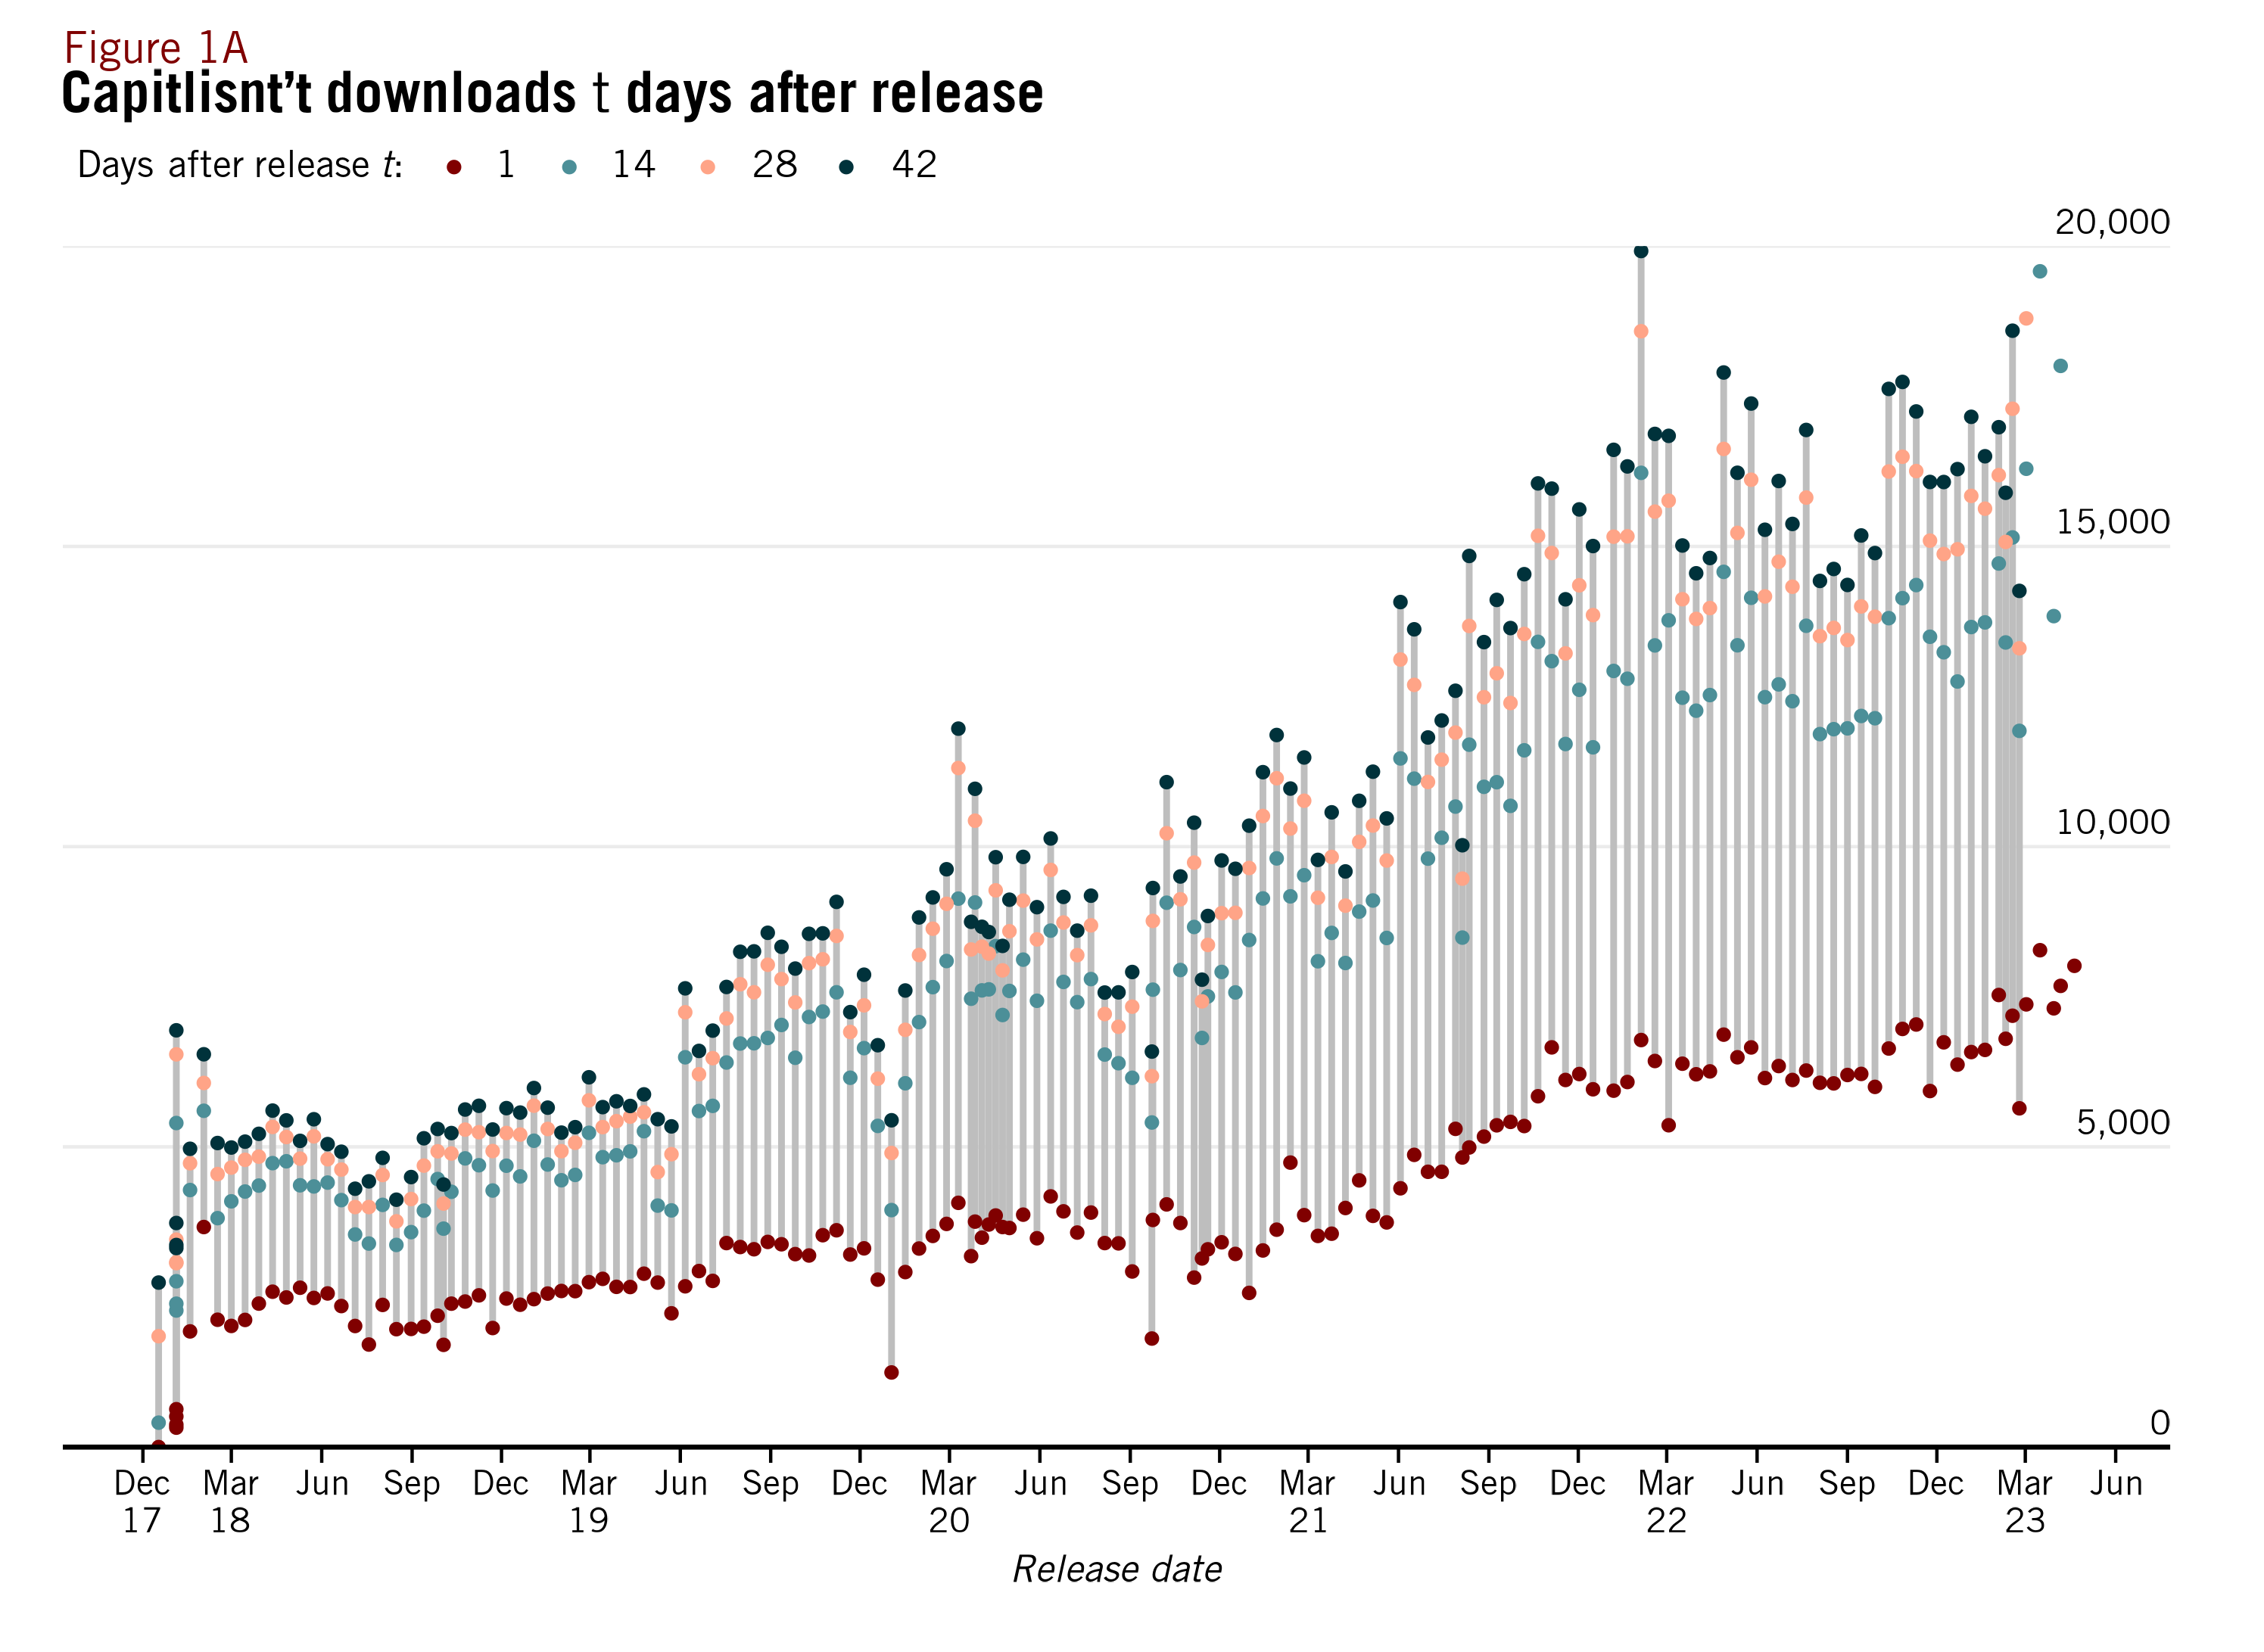
\includegraphics[width=0.9\textwidth]{figures/all_1142842_day_cumul_perf.png}
  \caption{}
  \label{fig:all_1142842_cumul_perf}
\end{figure}

Secondly, and perhaps more importantly, this is also clear in the mid-run performance of new episodes relative to old episodes. That is, even if listeners are not of the die-hard type, there are a growing number of listeners who are ``loyal'' (will eventually get around to the episode even if it isn't their highest priority). Though the logic for identifying the loyal listeners is fuzzier than that for identifying die-hard listeners, a number of mid-run phenomena constitute evidence for their growing number. Consider that for the first year of the podcast's run (between March 2018 and June 2019), the ``tail'' of episode downloads was almost constant as symbolized by the almost flat trend line that would run through all of the blue, 42-day downloads. However, following this period the ``growing'' barbell corresponds to greater gaps between first-, 14-, 28-, and 42-day downloads. These growing gaps suggest that listeners either a) continue to discover the podcast for the first time and listen to the back catalog; or b) have already discovered the podcast in the past, and are of the loyal type and will eventually get around to listening a given episode following its release. The widening of the barbell over time represents a growing loyal audience.\\

\begin{figure}[!htbp]
  \centering
  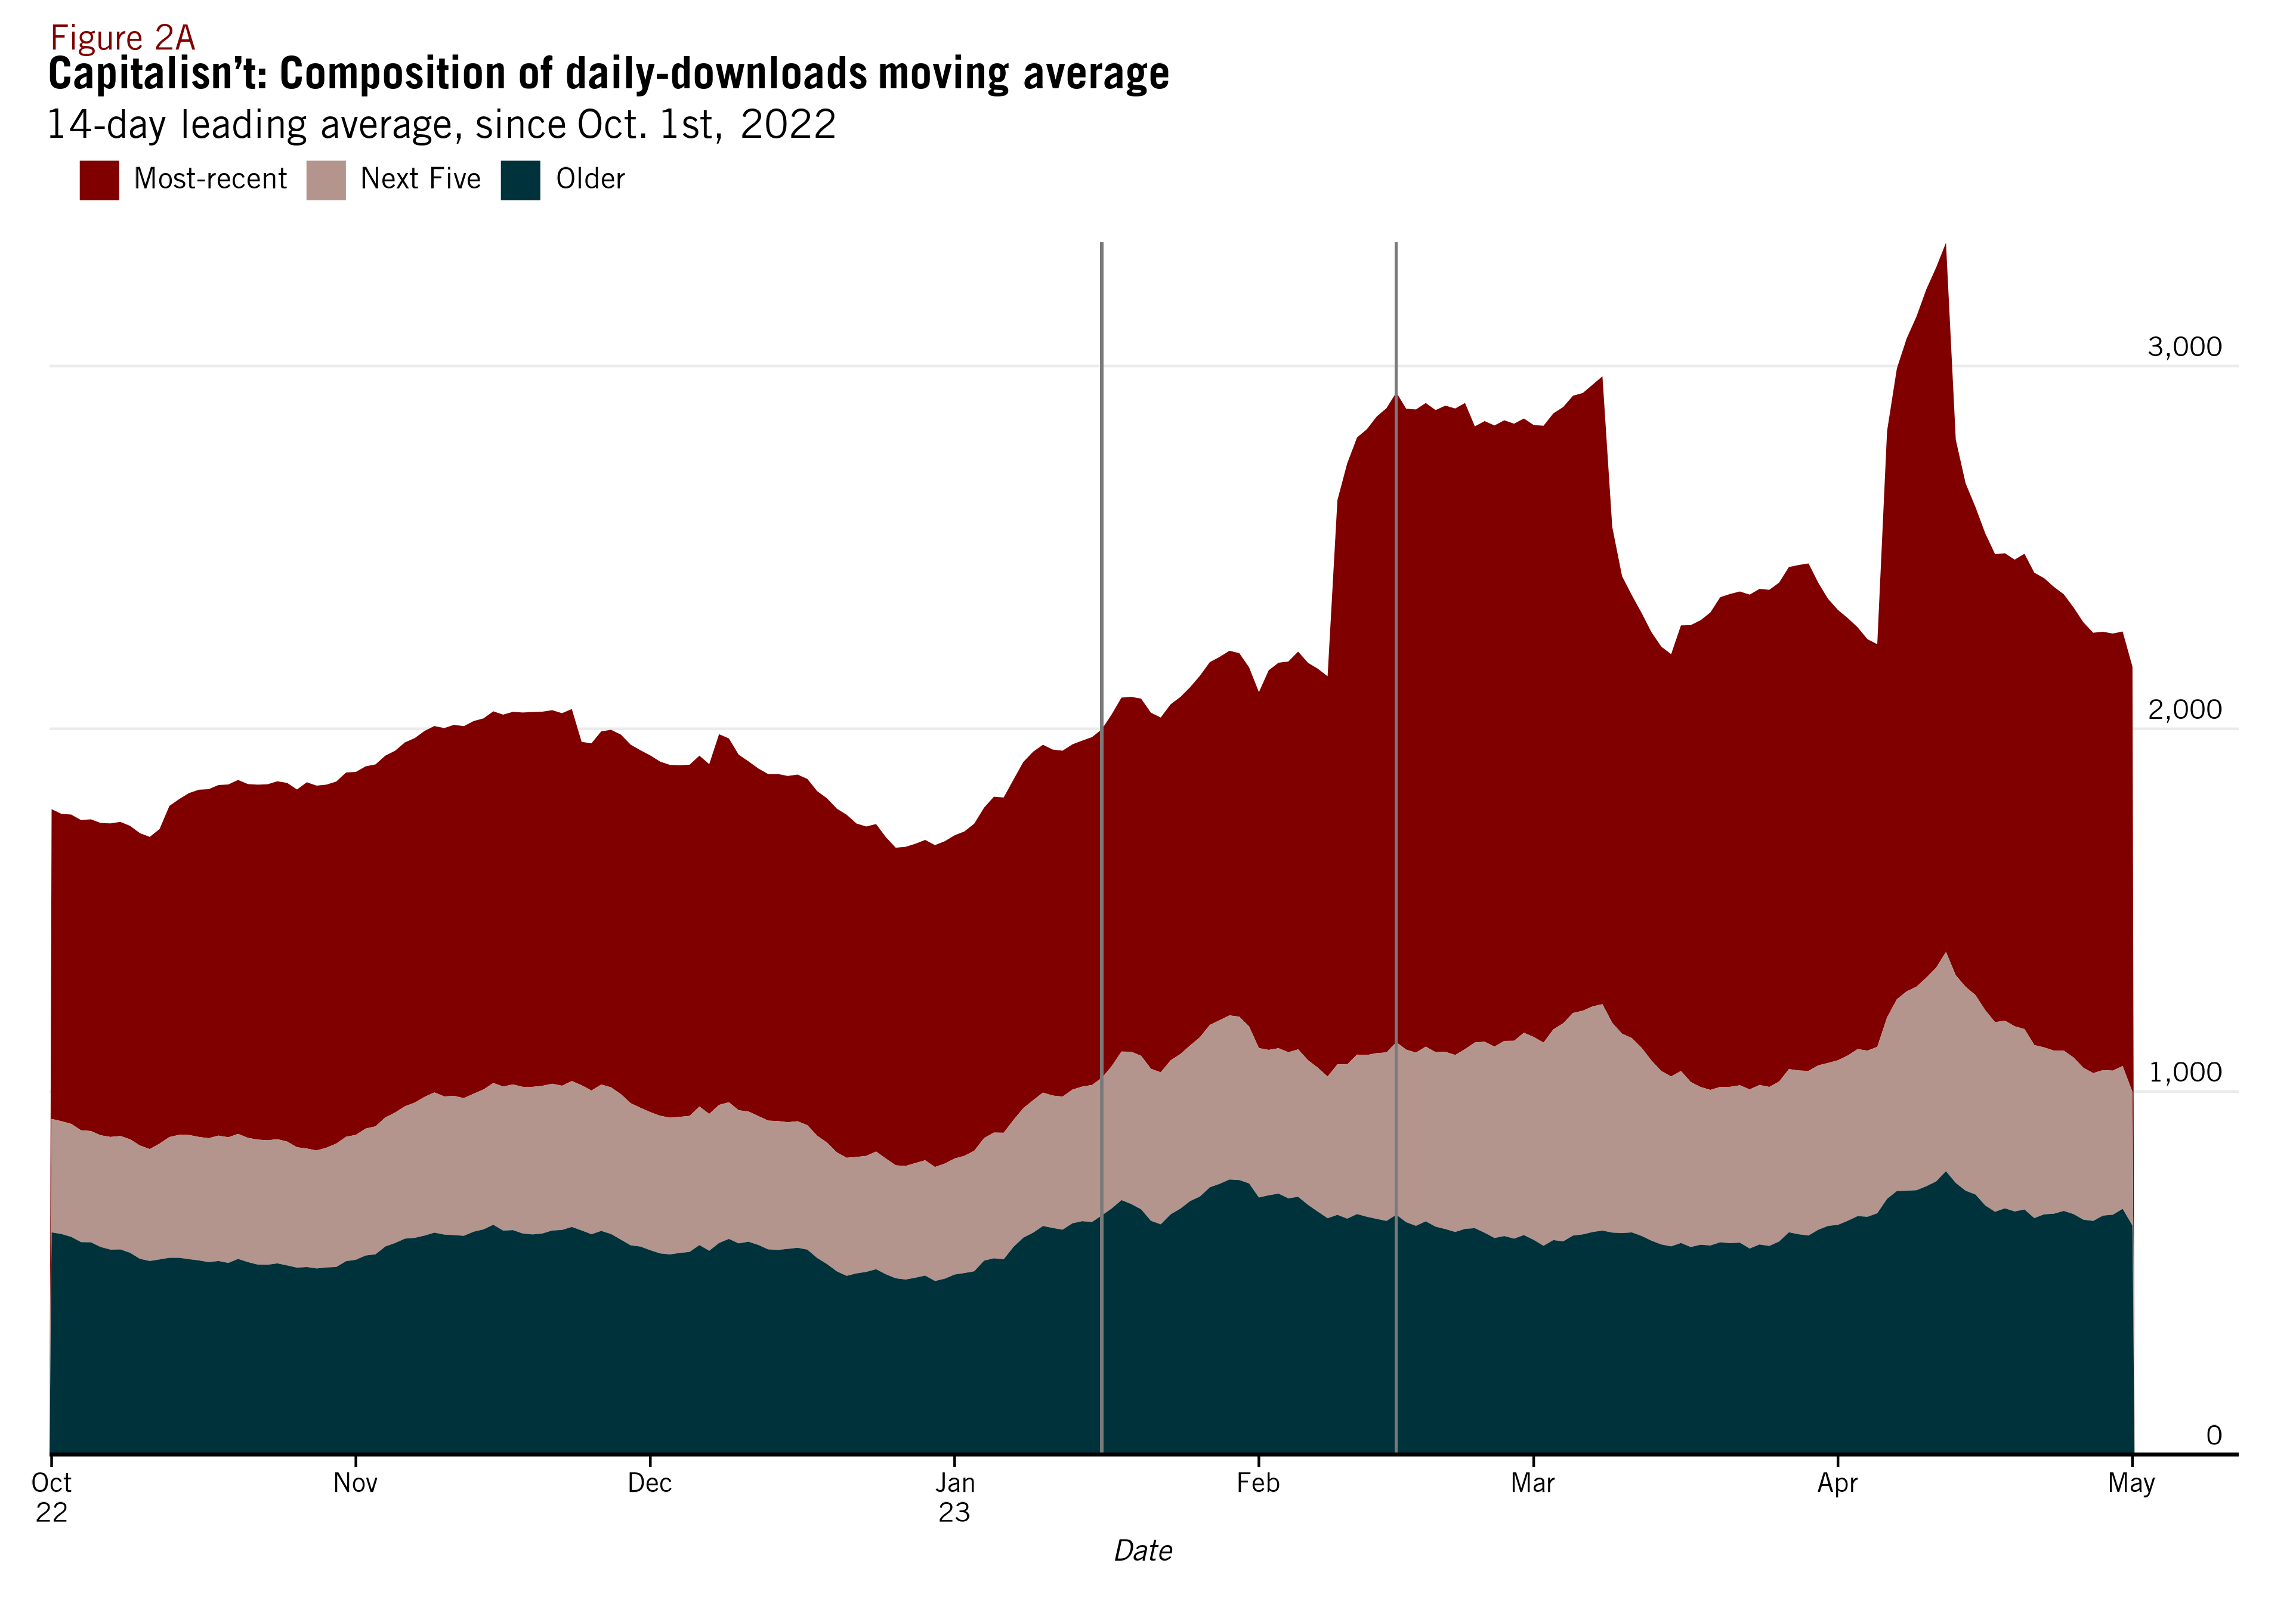
\includegraphics[width=0.9\textwidth]{figures/recent_podcast_moving_avg_decomp.png}
  \caption{}
  \label{fig:recent_moving_avg_perf_decomp}
\end{figure}

\begin{figure}[!htb]
  \centering
  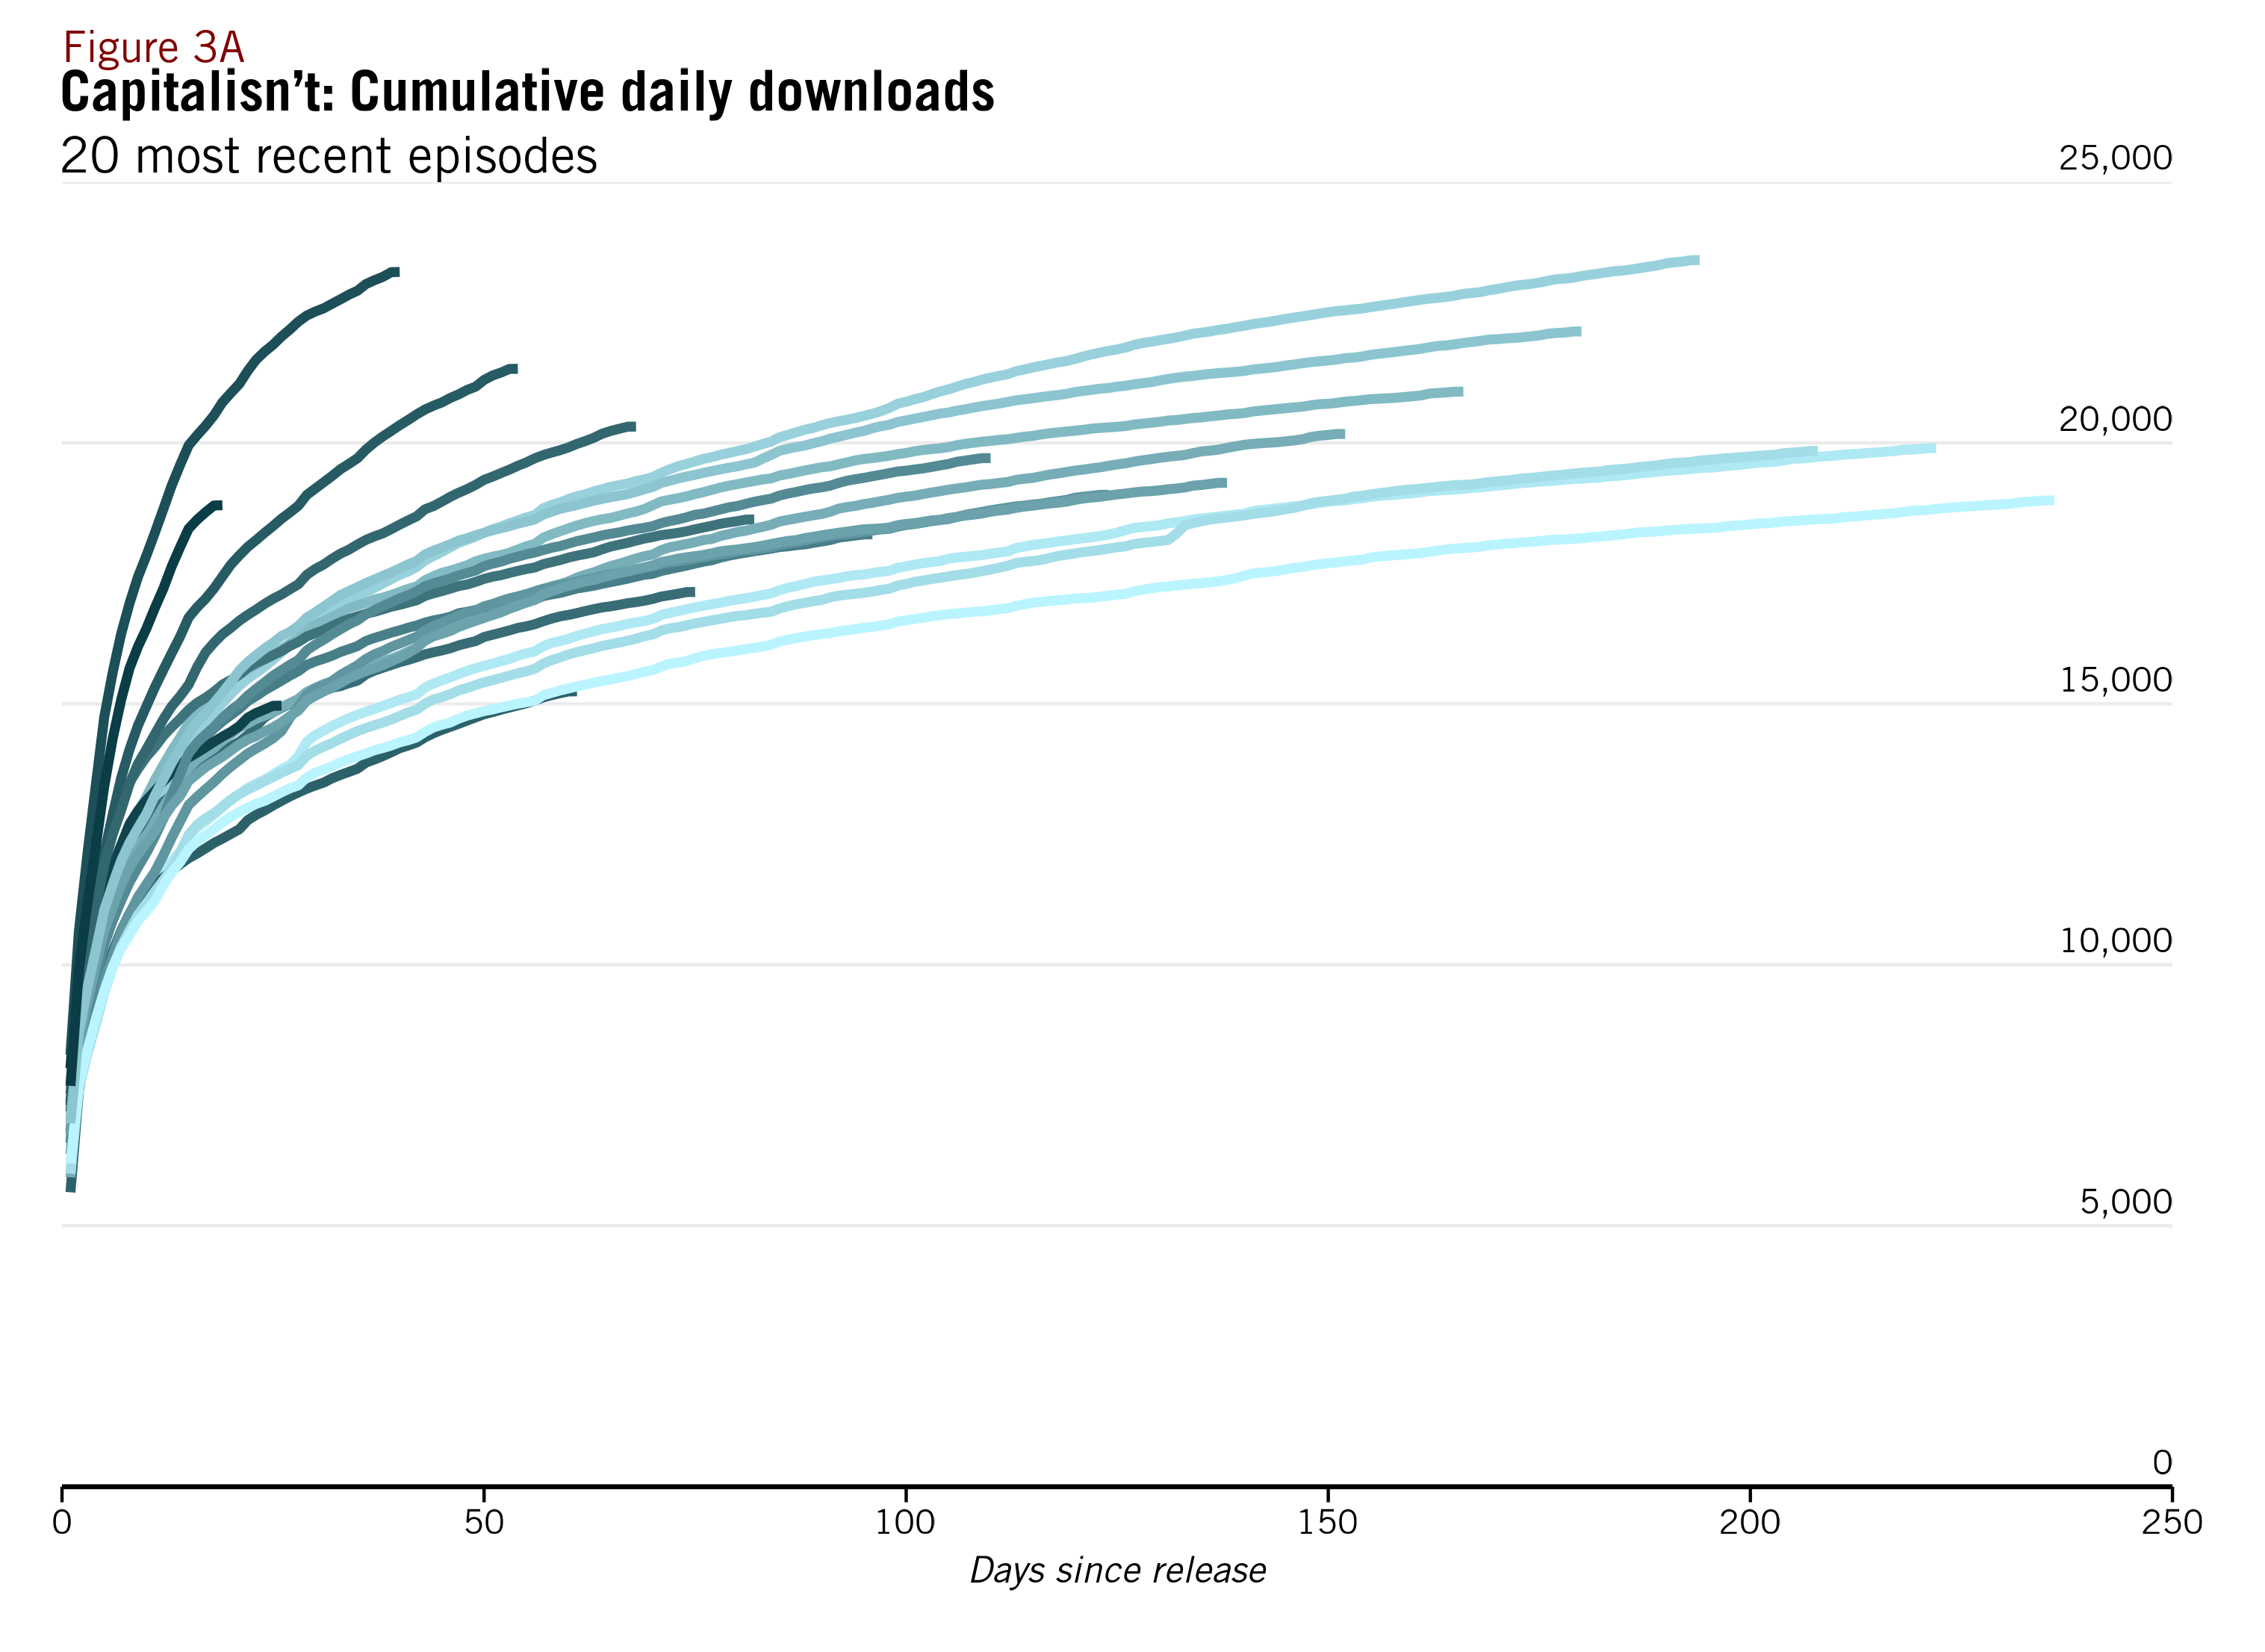
\includegraphics[width=0.9\textwidth]{figures/recent_20_episodes_cumul_perf.png}
  \caption{}
  \label{fig:recent_20_cumul_perf}
\end{figure}

The presence of this ``long-tail'' of downloads is further evidenced by Figures \ref{fig:recent_moving_avg_perf_decomp} and \ref{fig:recent_20_cumul_perf}.\footnote{Full-sample equivalents of these figures are available in the appendix.} In Figure \ref{fig:recent_moving_avg_perf_decomp}, the 14-day leading average --- a statistic selected to try to capture the performance of an episode while it is the most recently released episode for a biweekly release cadence --- of the podcast's cumulative (all episodes) downloads is decomposed into three parts: Most-recent, next five, and older. as expected, on any given day, the most-recently released episode constitutes a majority of downloads. However, the subsequent categories also constitute a non-negligible share of downloads suggesting that people continue to listen to the back-catalog of episodes. Additionally, note that whereas the most-recent episode download performance is relatively volatile due to the performance of \textit{only the current episode}, the performance of the back catalog is smoother.\footnote{This phenomenon is most pronounced during the period in late mid-February through March 2023 because the podcast briefly switched to a weekly release cadence (causing a mechanical increase in the 14-day leading average). The next-five, and older-episode downloads, however, are smoothed over a number of episodes.}\\

Figure \ref{fig:recent_20_cumul_perf} also exhibits the evolving performance of the podcast but at the episode level. Cumulative downloads are plotted on the vertical against days since release on the horizontal. Newer episodes are represented in darker shades of blue. The logarithmic shape of cumulative downloads is to be expected. The ``flattening'' of the curve against the vertical axis, however, represents better first-n-day performance of a given episode and the seemingly higher-valued asymptote that newer episodes' cumulative downloads approach represents a growing audience that consistently listens to the growing back-catalog of episodes.\\

In short, there appears to be a considerable weight of evidence that suggests that \textit{Capitalisn't} is a podcast that is growing over time, independent of paid-for advertising efforts. Thus, against this backdrop of secular growth, paid-for advertising would have to be justified by exceptional returns to expenditure.

\section{Policy Evaluation}
This section will report increasingly well-specified estimates of whether the WMATA advertising campaign had significant effects on the performance of the podcast.

\subsection{Naive Episode-Level OLS}
The most naive specification to test whether the ad campaign has an effect would test for whether cumulative downloads (at some point in time) are higher for episodes that are ``treated'' by the ad campaign than those that are not. An episode-level OLS estimation as decribed above may be specified as follows:

\begin{equation}
  \label{ep-level-naive-ols}
  \text{CumulativeDownloads}_i = \alpha + \beta_1\text{Advertisement}_i + X_i +\varepsilon_i, 
\end{equation}

where for each episode $i$, cumulative downloads would be estimated as a function whether or not an episode has experienced the Advertisement (a binary variable) treatment. Thus, we would expect $\beta_1$, the coefficient of interest, to be positive. In \eqref{ep-level-naive-ols}, $X_i$ is a vector of episode-level control variables that might also be correlated with cumulative downloads. The results of a series of OLS estimates of the above specification are presented in Table \ref{tab:ep-level-naive-ols}. In this table, Columns (1) through (3) present regression estimates where the dependent variable is episode-level cumulative downloads at 14 days following release. Columns (4) through (8) present estimates where the dependent variable is cumulative downloads 28 days following release. These definitions of performance are preferred because of the podcast's usual biweekly release cadence.\\

\begin{landscape}
  \begin{table}

\caption{Episode-level Naive OLS estimates \label{tab:ep-level-naive-ols}}
\centering
\begin{tabular}[t]{lcccccccc}
\toprule
\multicolumn{1}{c}{ } & \multicolumn{3}{c}{Cumul. Downloads ($t=14$)} & \multicolumn{5}{c}{Cumul. Downloads ($t=28$)} \\
\cmidrule(l{3pt}r{3pt}){2-4} \cmidrule(l{3pt}r{3pt}){5-9}
  & (1) & (2) & (3) & (4) & (5) & (6) & (7) & (8)\\
\midrule
Trailing Avg. ($n=5$, $t=14$) & \num{0.973}*** & \num{0.975}*** & \num{0.976}*** &  &  &  &  & \num{1.886}+\\
 & (\num{0.025}) & (\num{0.026}) & (\num{0.026}) &  &  &  &  & (\num{1.049})\\
Trailing Avg. ($n=5$, $t=28$) &  &  &  & \num{0.970}*** & \num{0.973}*** & \num{0.974}*** & \num{0.970}*** & \num{-0.672}\\
 &  &  &  & (\num{0.025}) & (\num{0.026}) & (\num{0.026}) & (\num{0.025}) & (\num{0.900})\\
WMATA Digital Ad &  & \num{-154.527} & \num{-177.062} &  & \num{-309.120} & \num{-318.683} &  & \\
 &  & (\num{862.108}) & (\num{863.439}) &  & (\num{977.589}) & (\num{978.589}) &  & \\
Economist/Vox Ad &  &  & \num{-390.021} &  &  & \num{-255.310} &  & \\
 &  &  & (\num{507.944}) &  &  & (\num{988.521}) &  & \\
Intercept & \num{25.588} & \num{16.324} & \num{17.376} & \num{71.318} & \num{52.647} & \num{52.174} & \num{71.318} & \num{-68.605}\\
 & (\num{204.117}) & (\num{209.260}) & (\num{209.707}) & (\num{220.592}) & (\num{226.559}) & (\num{226.932}) & (\num{220.592}) & (\num{280.956})\\
\midrule
Num.Obs. & \num{148} & \num{148} & \num{148} & \num{147} & \num{147} & \num{147} & \num{147} & \num{147}\\
R2 & \num{0.939} & \num{0.939} & \num{0.939} & \num{0.937} & \num{0.937} & \num{0.937} & \num{0.937} & \num{0.940}\\
R2 Adj. & \num{0.938} & \num{0.938} & \num{0.938} & \num{0.937} & \num{0.936} & \num{0.936} & \num{0.937} & \num{0.939}\\
\bottomrule
\multicolumn{9}{l}{\rule{0pt}{1em}+ p $<$ 0.1, * p $<$ 0.05, ** p $<$ 0.01, *** p $<$ 0.001}\\
\multicolumn{9}{l}{\rule{0pt}{1em}Standard errors presented in parentheses are heteroskedastic-robust errors}\\
\end{tabular}
\end{table}

\end{landscape}

Though the regression estimates presented in Table \ref{tab:ep-level-naive-ols} do not exhibit statistical significance for either the WMATA or Economist/Vox Ad campaign indicator variables, the ``Trailing Average'' regressors exhibit high levels of statistical significance across specifications.\footnote{These regressors are constructed as the the average cumulative downloads of the previous five ($n=5$) episodes 14 ($t=14$) or 28 days ($t=28$) following release.} Notably, the central point estimates are all less than 1 (Column (8) results are explicated at greater length below). This would suggest that podcast performance as defined by the relevant dependent variable is \textit{decaying} over time. For example, in the terms of the estimates presented in Column (1), an episode's cumulative downloads 14 days following release is approximately 97.4\% of the average of the previous five episodes at the same time following their own releases. This runs counter to the story represented by the summary statistics and motivating figures above: that there appears to be a largely secular pattern of growth in downloads (consider the upward trend of light-blue points in Figure \ref{fig:all_1142842_cumul_perf}). Note however, that for all of these coefficient estimates, 1 lies on or within the 95\% confidence interval.\\

In fact, the average upper-bound of the confidence intervals for the Trailing Average regressor in these 7 specifications is 1.002. A 2\% growth rate relative to the average of the previous 5 episodes suggests a doubling time of approximately 35 periods. With a biweekly release cadence, this corresponds to approximatley 1 year and 5 months, not entirely inconsistent with the growth that is visually described in Figure \ref{fig:all_1142842_cumul_perf}. Of course, the confidence interval on the central point estimates also includes values considerably below 1. This is consistent with the performance of the podcast not monotonically improving. On balance, I would contend that these estimates are weak evidence of the podcast's growth over time.\\


The ``WMATA Digital Ad'' and ``Economist/Vox Ad'' regressors are both indicator variables that are coded as 1 if the episode was aired during either of these treatment periods. In short, they exhibit no meaningful degree of statistical significance. That is, after controlling for the growth of the podcast over time with the Trailing Average regressor, the advertisement campaigns do not appear to be predictive of higher cumulative downloads for treated episodes, as one might hypothesize. This is further tested in other specifications below. Column (8) in Table \ref{tab:ep-level-naive-ols} is included as another test of the podcast's serial autocorrelation with itself (at the episode-level). Note that both of the Trailing Average regressors exhibit (at varying levels of statistical significance). The 14-day regressor appears to be both very statistically significant and very positive and greater than 1. The coefficient is on the 28-day regressor however, is statistically significant at the 10\% level and negative. Both of these coefficients have very large conffidence intervals but the summation of the two suggest a time-trend that is positive, consistent with the evidence presented above.

\subsection{Regression Kinks}
\begin{figure}[!htb]
  \centering
  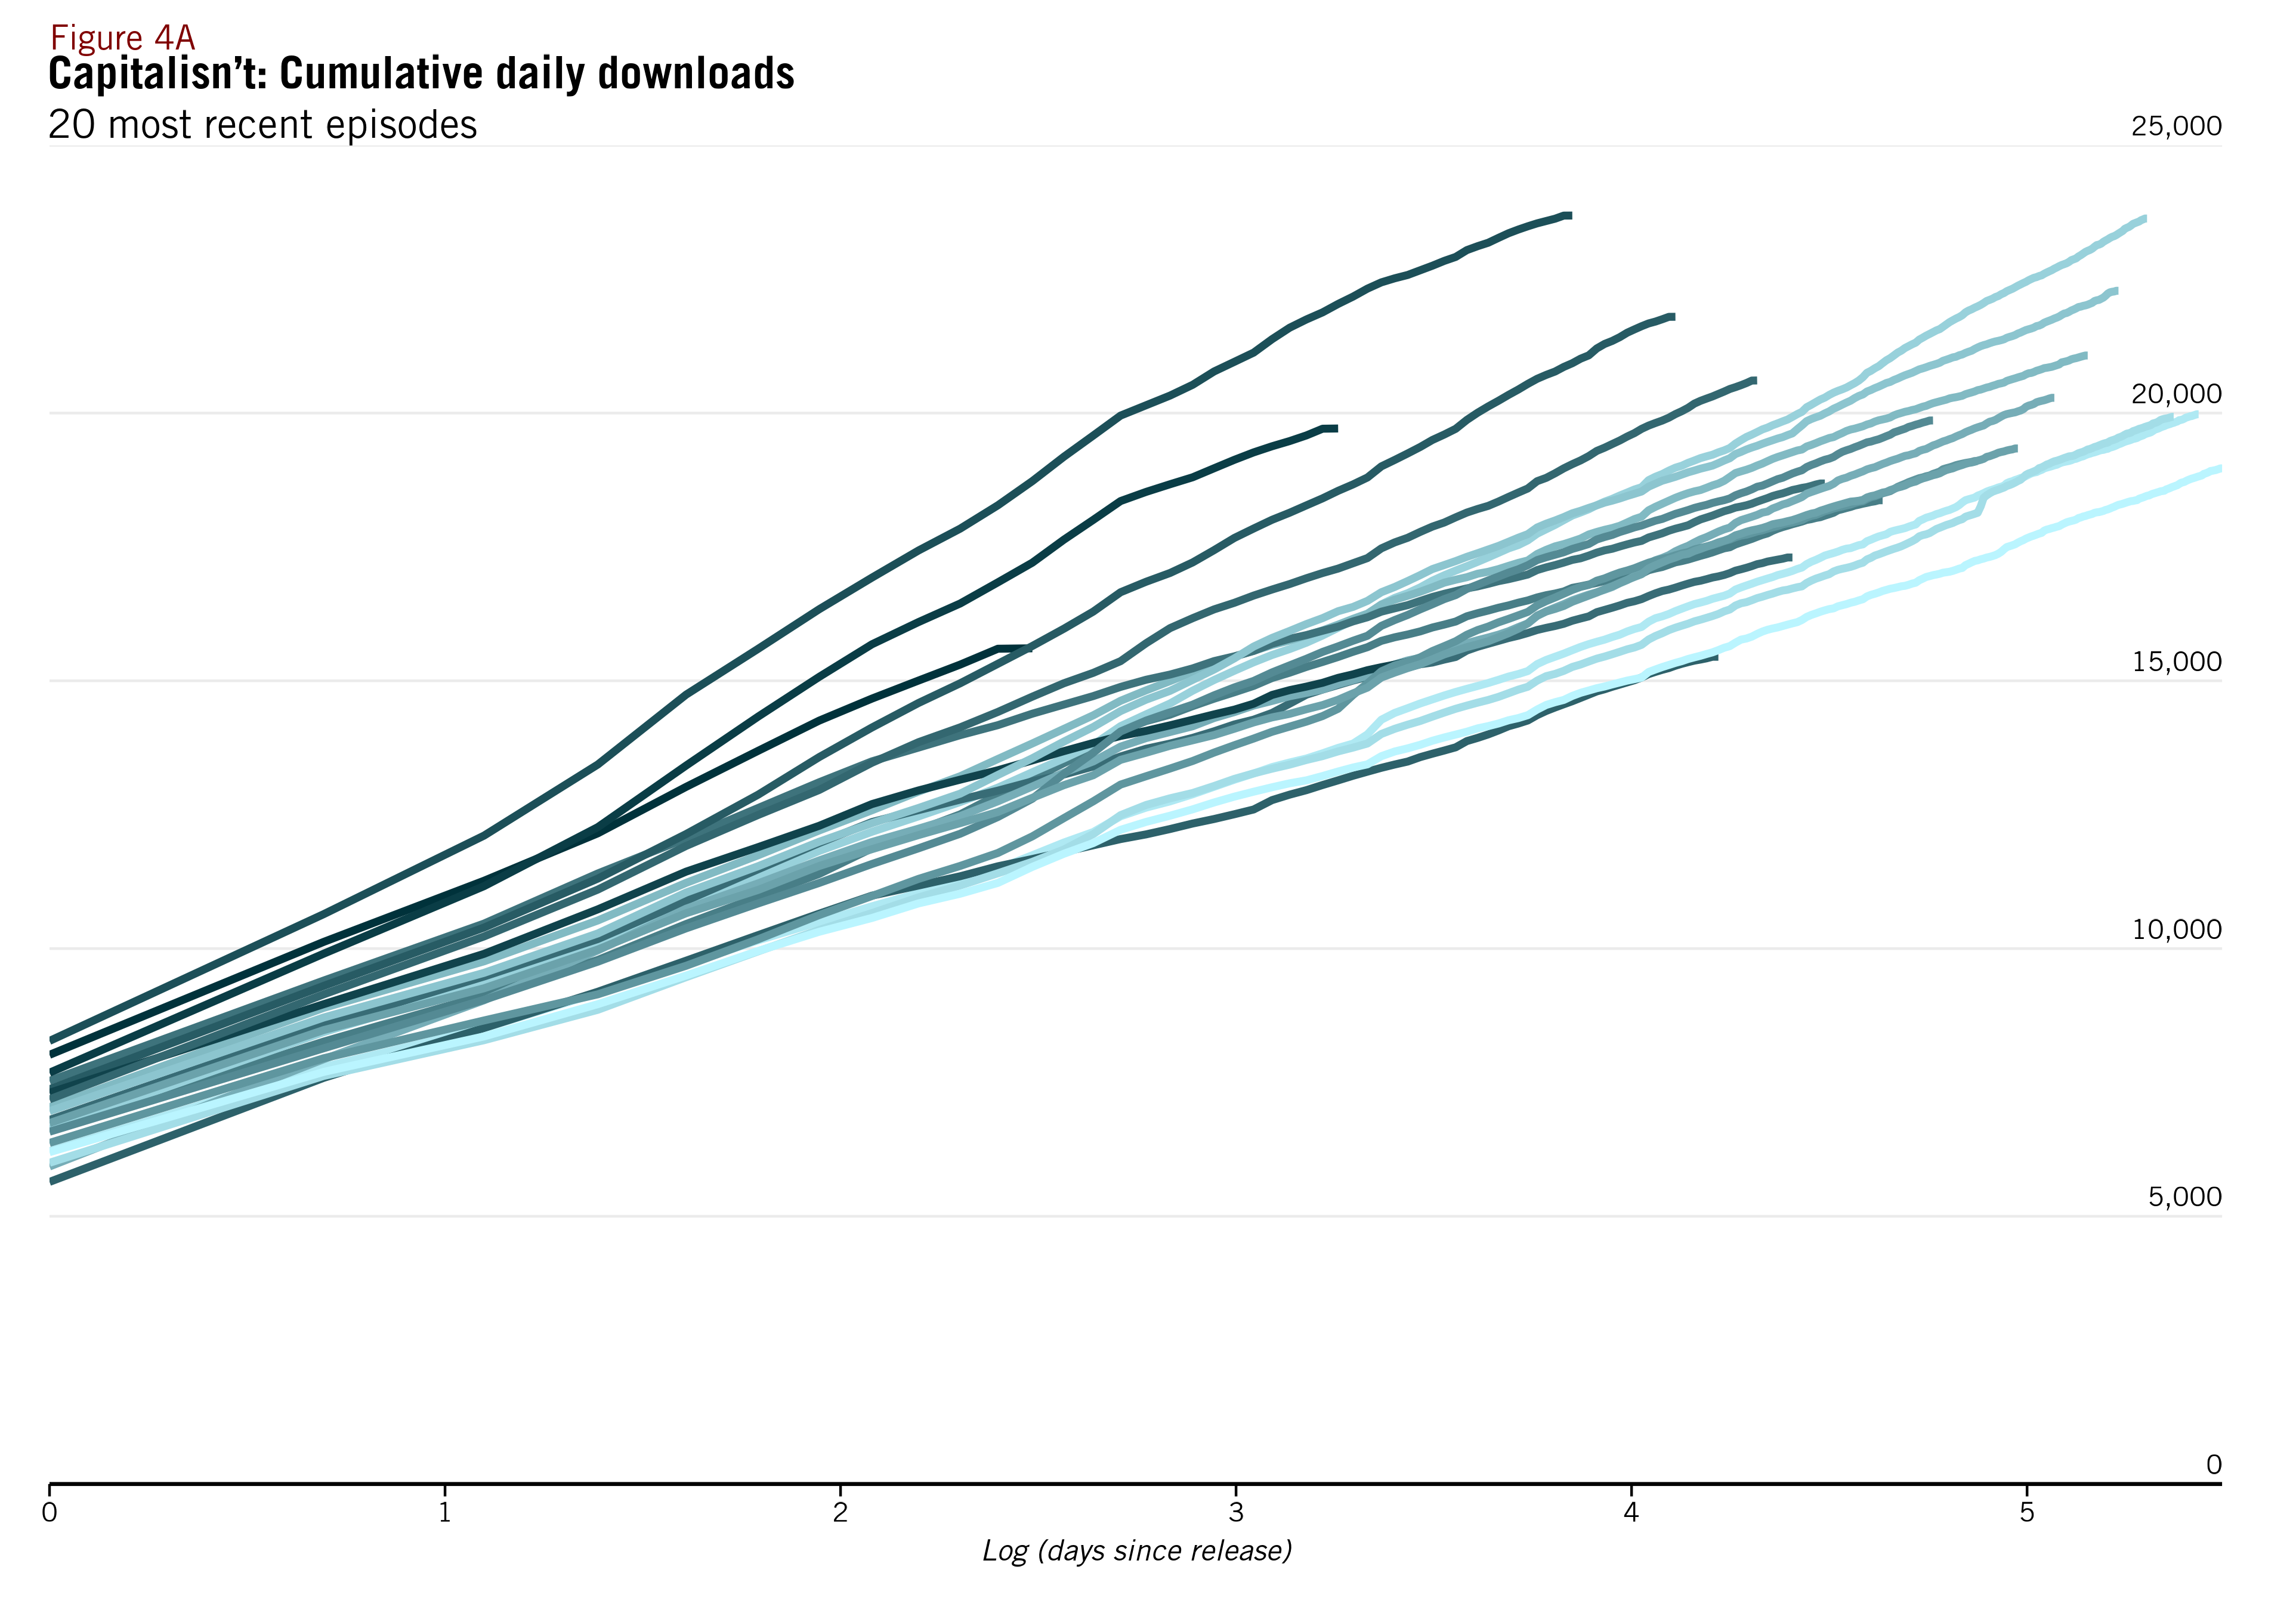
\includegraphics[width=0.9\textwidth]{figures/recent_20_episodes_linear_cumul_perf.png}
  \caption{}
  \label{fig:recent_20_linear_cumul_perf}
\end{figure}

As demonstrated by Figure \ref{fig:recent_20_cumul_perf} and Figure \ref{fig:recent_20_linear_cumul_perf}, the linearized equivalent, most performance ``trajectory'' of most episodes is remarkably predictable. Cumulative downloads exhibit a logarithmic (daily downloads exhibit an exponential decay) behavior. One way of assessing the efficacy of the WMATA ad campaign would be to test if, on days in which the advertisement is in effect, podcast performance statistically significantly deviates from this otherwise predictable trajectory.\\

I attempt to operationalize this at the podcast and episode levels. Identifying a ``kink'' in podcast performance around the advertising campaign in an OLS setting can be done as follows:

\begin{align}
  \label{kink-ols}
    \text{CumulativeDownloads}_i &= \alpha + \beta_1\log{\text{DaysSinceRelease}}_i + \beta_2\text{Adv}_i\\ \nonumber
      & +\beta_3(\log{\text{DaysSinceRelease}} \times \text{Adv})_i + X_i + \varepsilon_i
\end{align}

Here, the interpretation of the estimated coefficients are quite intuitive: $\alpha$ represents estimated first-day downloads ($\log(1)=0$). $\beta_1$ captures the linear slope that describes the performance trajectory of an episode. Because Adv is an indicator variable for whether the observation (daily frequency cumulative downloads) is treated by advertising, $\beta_2$ can be thought of as the step-wise increase in the number of downloads that the unit of observation experiences at the beginning of the advertising period (more on the interpretation of this coefficient below). In \eqref{kink-ols}, $\beta_3$ is the coefficient of interest and represents the magnitude of the interaction term between the $\log$DaysSinceRelease explanatory variable and the advertising treatment. Under the intuitive hypothesis that advertising should have a positive effect on daily downloads, the sign on this coefficient is expected to be positive. A statistically significant, positive $\beta_3$ estimate would imply that advertising \textit{does} have an effect and improves podcast performance relative to the its pre-advertising trajectory. $X_i$ is a vector of control variables (largely unavailable in our data setting) and $\varepsilon$ represents an error term.\\

Throughout \eqref{kink-ols} terms are assigned the entity sub-script $i$. Entities however, can be specified at the podcast or episode levels. The implications of this are manifold but I restrict my attention to episode-level analysis. Additionally, if we estimate \eqref{kink-ols} for all episodes simultaneously we suffer from sources of bias beyond those that are present in other estimates.\footnote{See section INSERT SECTION NUMBER REFERENCE HERE for more information on shortcomings} In particular, because the advertisement period is fixed in real terms (calendar dates), treatment in relative terms (note that this specification uses a relative days-since-release measure as a regressor) is staggered. So, for purposes of econometric simplicity, we estimate this model separately for each episode.\\

For illustrative purposes, consider Figure \ref{fig:tswift_fitted}, which plots the cumulative downloads of against the logarithm of days since release for the episode, ``Taylor Swift, Ticketmaster, and Chokepoint Capitalism with Cory Doctorow,'' release on December 12, 2022. The lines represent the fitted values estimated by \eqref{kink-ols} for this episode. This is an ideal episode to consider because it was release prior to the beginning of the advertising period and so had an established ``trajectory'' prior to being treated. The advertising period is plotted in blue whereas untreated observations are plotted in red.\\
 
\begin{figure}[!htb]
  \centering
  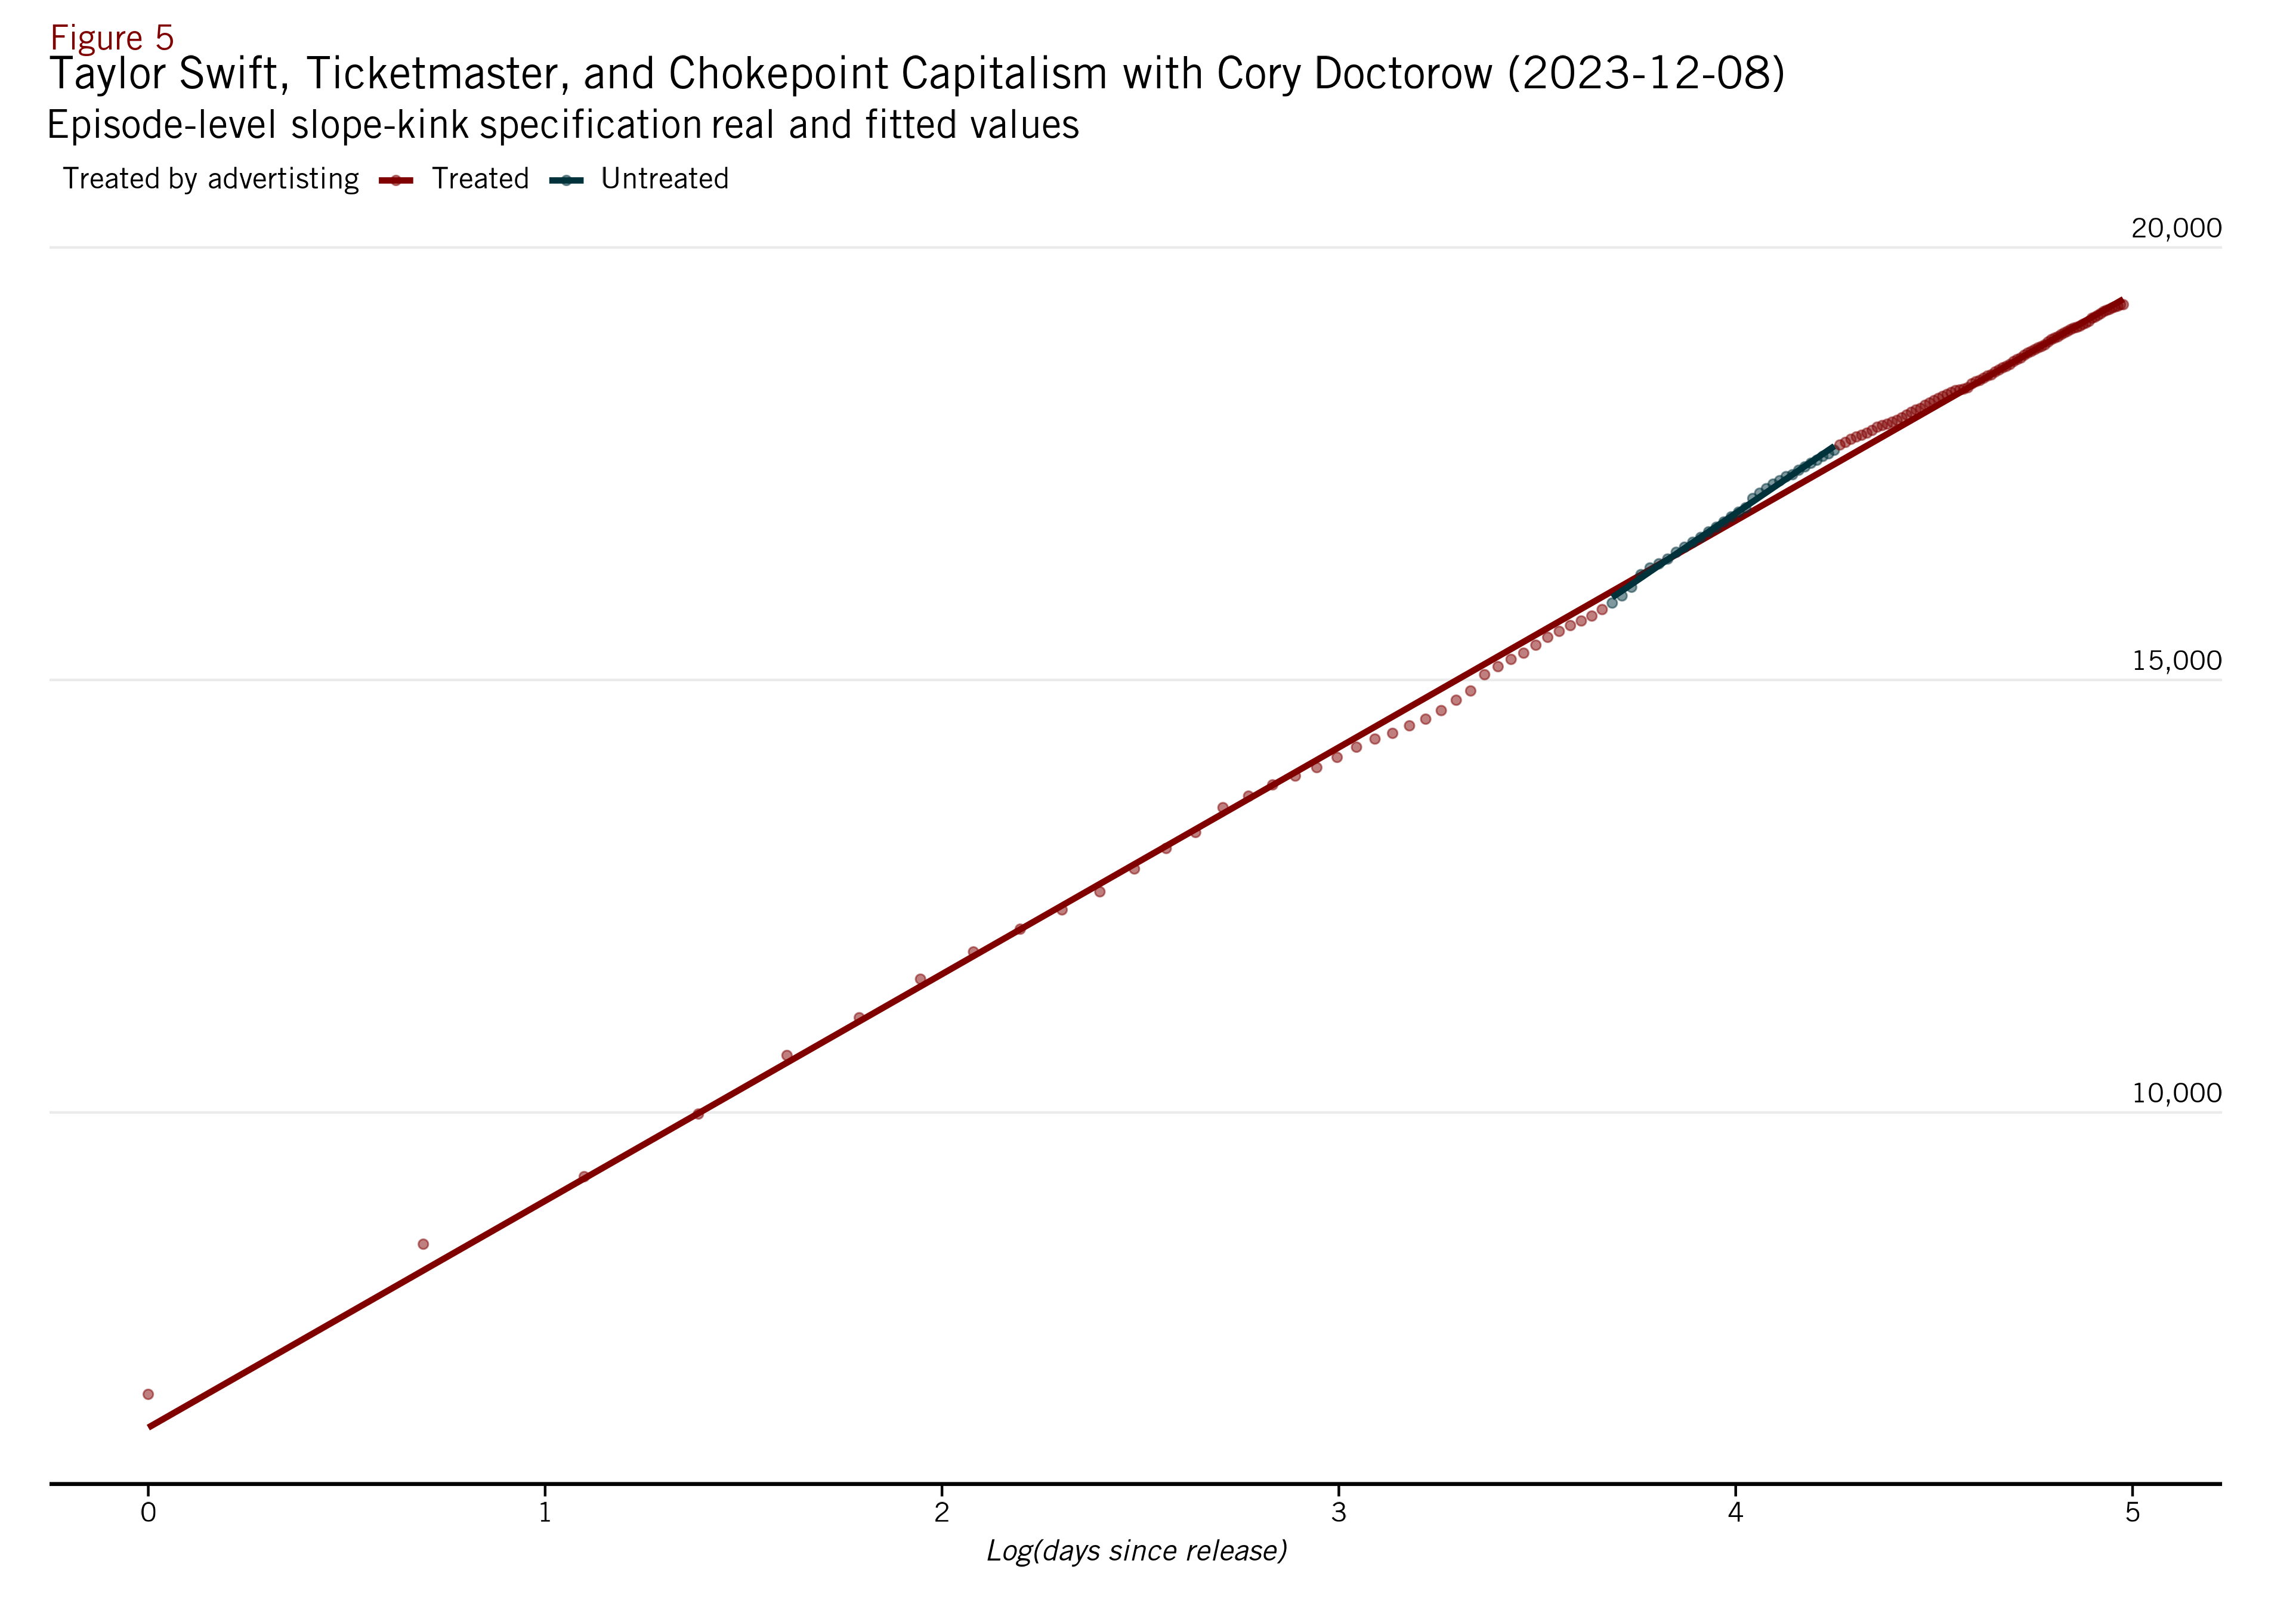
\includegraphics[width=0.9\textwidth]{figures/tswift_daily_kink_plot.png}
  \caption{}
  \label{fig:tswift_fitted}
\end{figure}
  
Note that for the advertising period, the slope of the fitted line is slightly greater than for the untreated period. Indeed, closer inspection of the particular models that the coefficient on th  interaction term, $\beta_3$, is in fact statistically significantly positive. The magnitude on the coefficient is small but this warrants closer inspection.\\

Generalizing this investigation, I re-esitmate \eqref{kink-ols} for the 50 most recent episodes (as those being plausibly treated by the advertising campaign); that is, episodes released since mid-July 2021. For such episode-specific regression, the sign and statistical significance of the estimated coefficients are plotted in a heatmap, as in Figure \ref{fig:kink-ols-heatmap}.\\ 

\begin{figure}
  \centering
  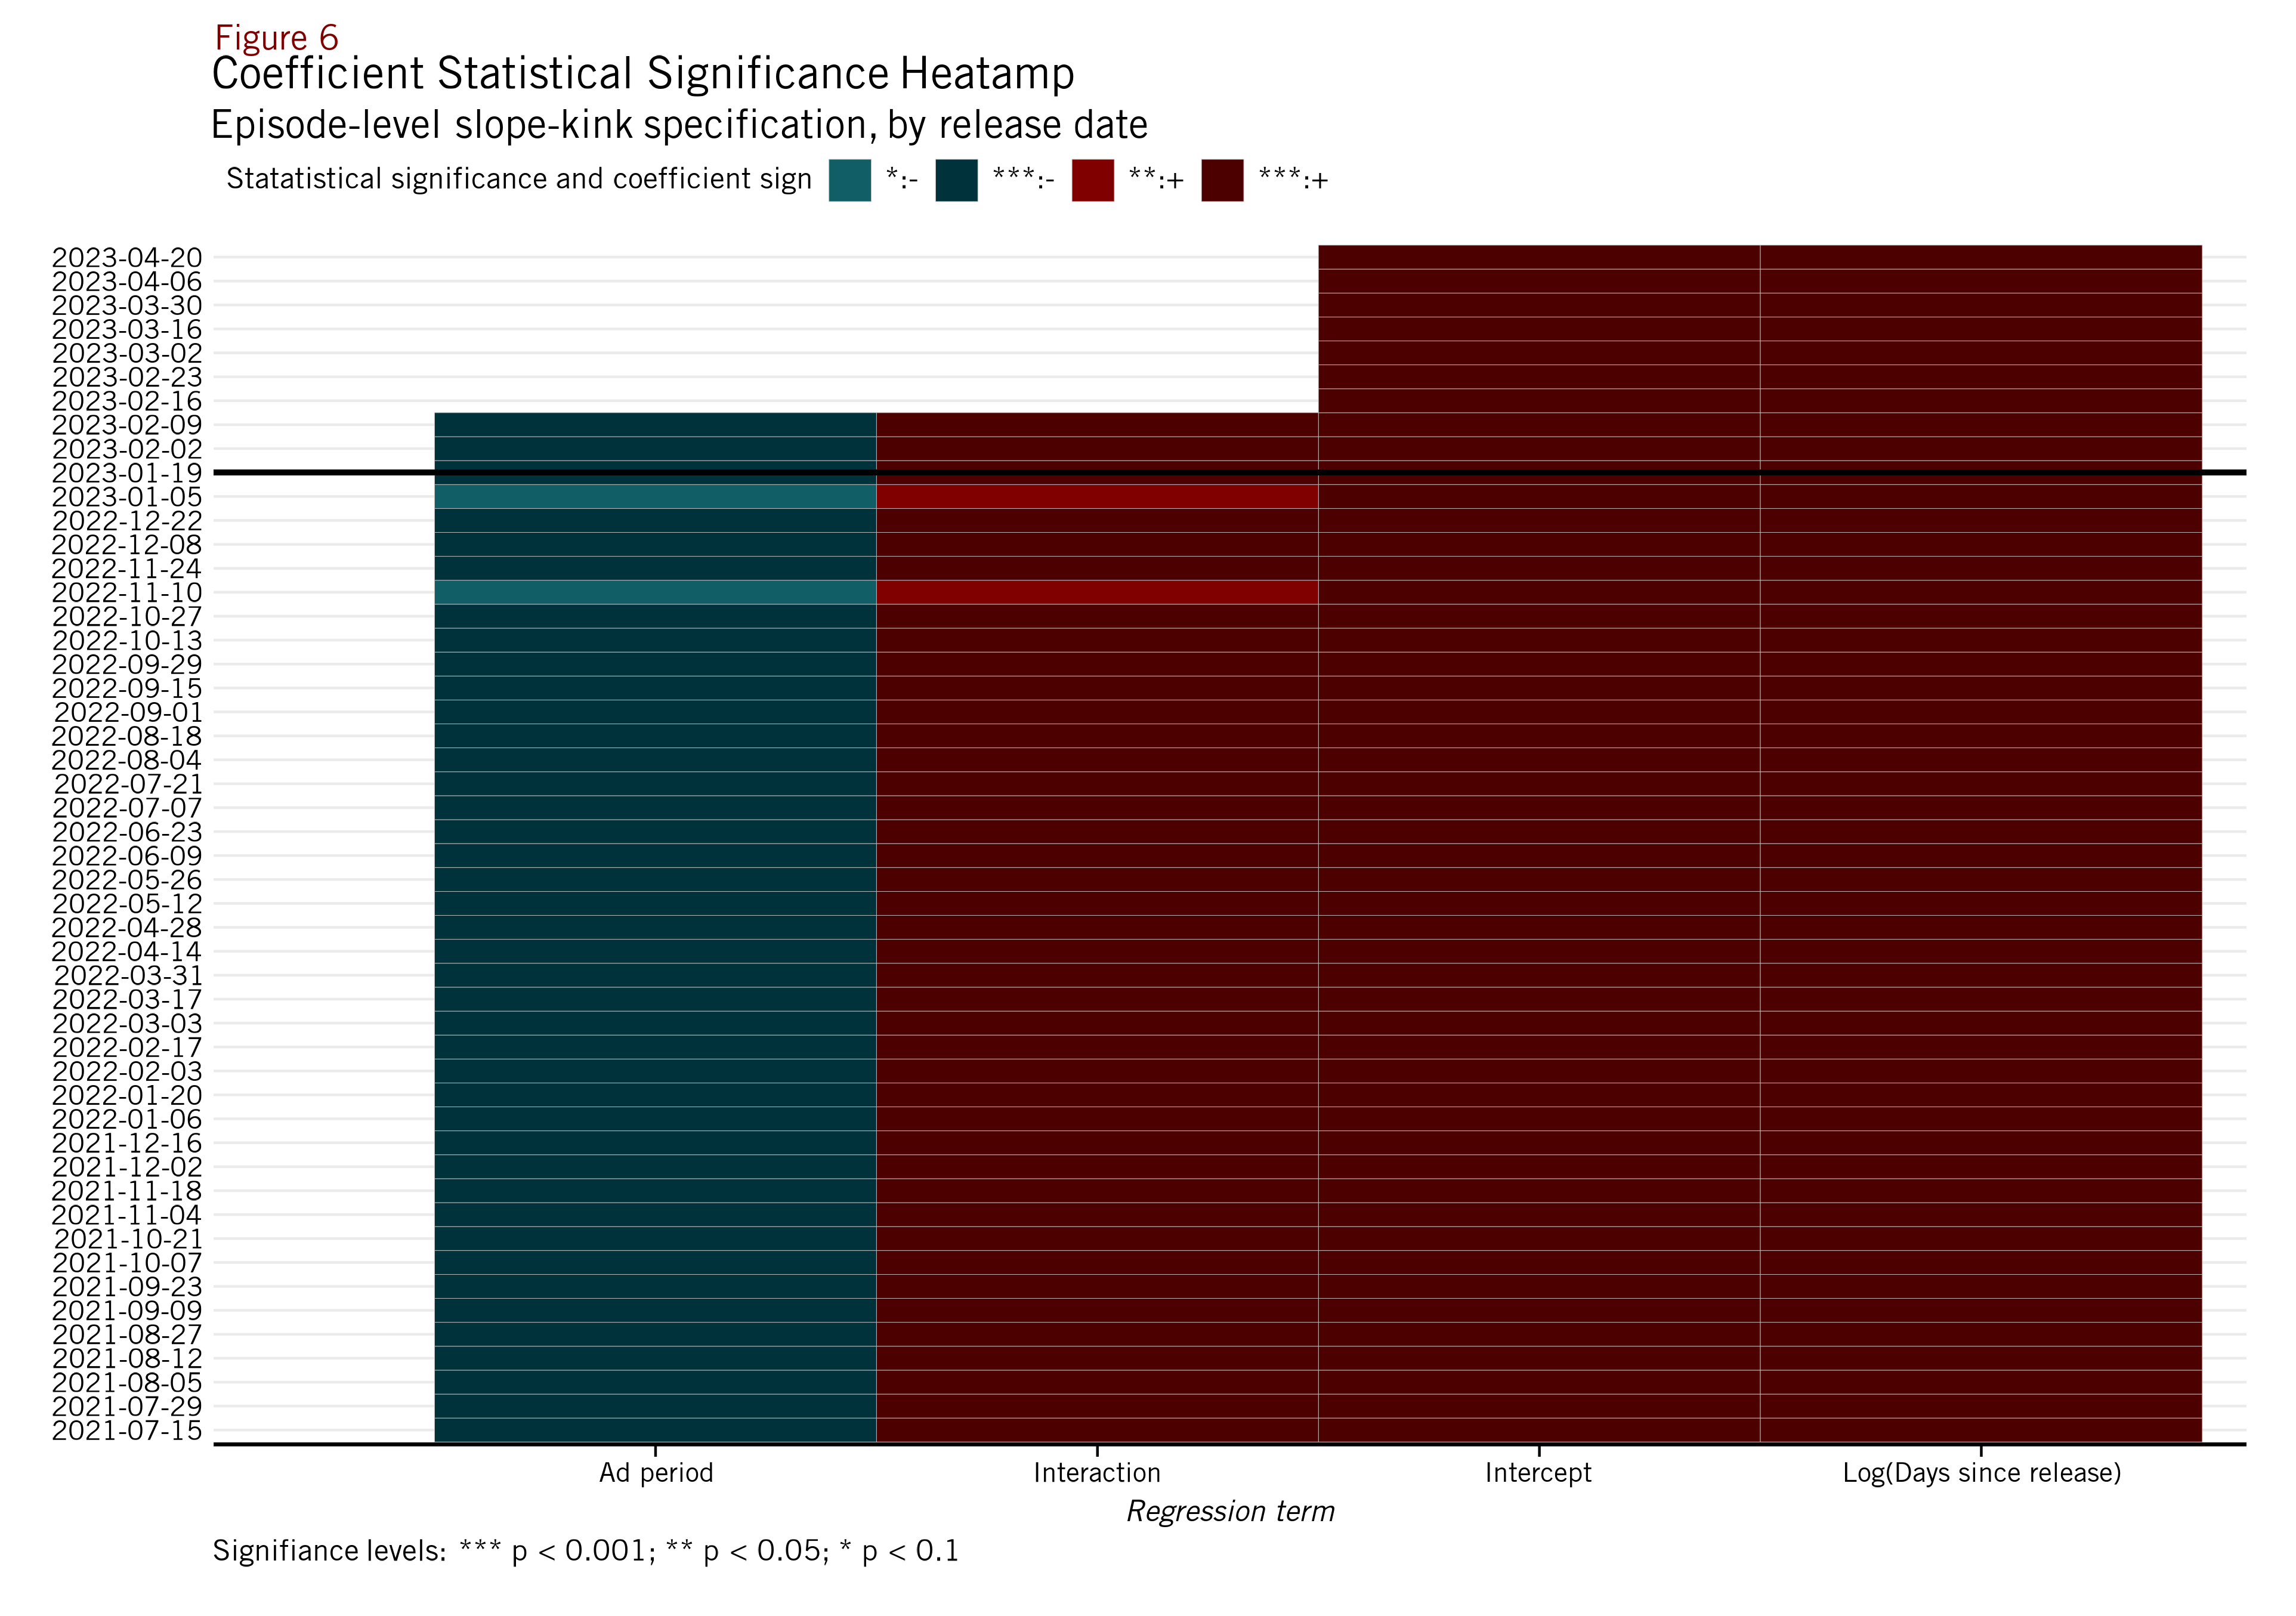
\includegraphics[width=0.9\textwidth]{figures/daily_kink_sig_heatmap.png}
  \caption{}
  \label{fig:kink-ols-heatmap}
\end{figure}

These results appear prima facie encouraging. For almost every episode, the relevant $\beta_3$ coefficient on the interaction appears to be statistically significant and positive. A naive event-study style interpretation of these results suggests that the advertisement campaign was at least superficially effective: it caused downloads to increase relative to the expected trajectory for effectively every episode.\footnote{The statistically significant negative coefficient on the advertisement regressor is not of particular concern. That is, because of the regression design, fitting a second line with a greater slope to a sample of points relatively far away from the vertical axis ($\log \text{DaysSinceRelease}=0$). That is, this negative ``intercept'' value is sufficiently small to be offset by the large estimated value of $\hat{\beta_1}\times\log\text{DaysSinceRelease}$ so that on the boundary of the advertisement period beginning, the line that fits the treated period intersects the line that fits the untreated observations.} \\

However, this interpretation is flawed due to potentially attributing a spurious increase, perhaps driven by some unobserved variable, to the advertising treatment. In fact this is quite likely given that towards the end of the advertising period, the podcast briefly switched to a weekly release cadence, potentially increasing the apparent performance of episodes due simply to new listeners (attracted to the podcast due to secular growth associated with publishing episodes more regularly) perusing the back catalog of episodes. So, additional analysis is required.

\subsection{DMV Diff-in-Diff}
In addition to provide daily temporal resolution, the Simplecast API also provides a relatively high degree of geographic resolution to downloads data. Simpelcast provides an API endpoint that returns the at-present cross-sectional cumulative downloads data at the sub-state-location level throughout the United States. In order to construct a panel of episode-location-daily downloads data, I queried the API every day at midnight.\\

Using this panel, I am able to test the effectiveness of the advertising campaign not only in time (as the previous kink specification described by \eqref{kink-ols}), but also in space. The WMATA advertising was placed in stations throughout Washington, D.C., and in trains that moved throughout the greater D.C-Maryland-Virginia (DMV) area. Consequently, we treat downloads in these places as ``treated'' observations and other places throughout the United States as ``untreated'' units.\footnote{Simplecast does offer a relatively high degree of spatial resolution, usually, below the metropolitcan statistical area (MSA) level. For example, in Illinois, Chicago and Evanston are identified as two distinct places. However, it is unclear how Simplecast defines the boundaries between places (it does not, for example, use a county-based definition). By inspection, however, it does appear that all identified places are disjoint of each other.} We aggregate these small locations across state lines into a single ``DMV'' unit and leave all other places as untreated.\footnote{See Appendix INSERT APPENDIX HERE for a list of places identified as ``DMV'' places.}\\

I use a difference-in-differences (DID) estimation strategy to isolate the hypothesied effect of advertising on downloads. The intuition to this strategy is similar to that of regression-kink design. However, with location data, I am able to use untreated locations as a ``control'' group against which I can compare the change in the growth in cumulative downloads expected due to the advertising. A regression equation of this kind would be specified as follows:

\begin{align}
  \label{dmv-did}
  \text{CumulativeDownloads}_{ij} &= \alpha + \beta_1 \log \text{DaysSinceRelease}_{ij} + \beta_2 \text{Adv}_{ij} + \beta_3 \text{DMV}_i \\ \nonumber
    &+ \beta_4(\log \text{DaysSinceRelease} \times \text{DMV})_{ij} + \\ \nonumber
    &+ \beta_5(\log \text{DaysSinceRelease} \times \text{DMV} \times \text{Adv})_{ij} + X_i + \varepsilon_{ij} 
\end{align}

In \eqref{dmv-did}, $\text{DMV}_{ij}$ is an indicator variable that is coded as 1 if the location $j$ is in the treated DMV group. Additionally, $\beta_5$ is the coefficient of interest and is expected to be positive.\footnote{In contrast to many DID strategies, there are no ``time'' subscripts, $t$ on regressors because we control for time as its own regressor. Additionally, I do not consider the possibility that places that are defined as never-treated (outside the DMV) could see an improvement in podcast performance due to the advertising. For the purposes of this investigation, I am not particularly concerned about spillover effects jeopardizing the identification startegy.} Similar to Figure \ref{fig:tswift_fitted}, Figure \ref{fig:yannelis-did-RoUS} provides an illustrative example of the intuition undergirding this estimation strategy.\\

\begin{figure}[!htb]
  \centering
  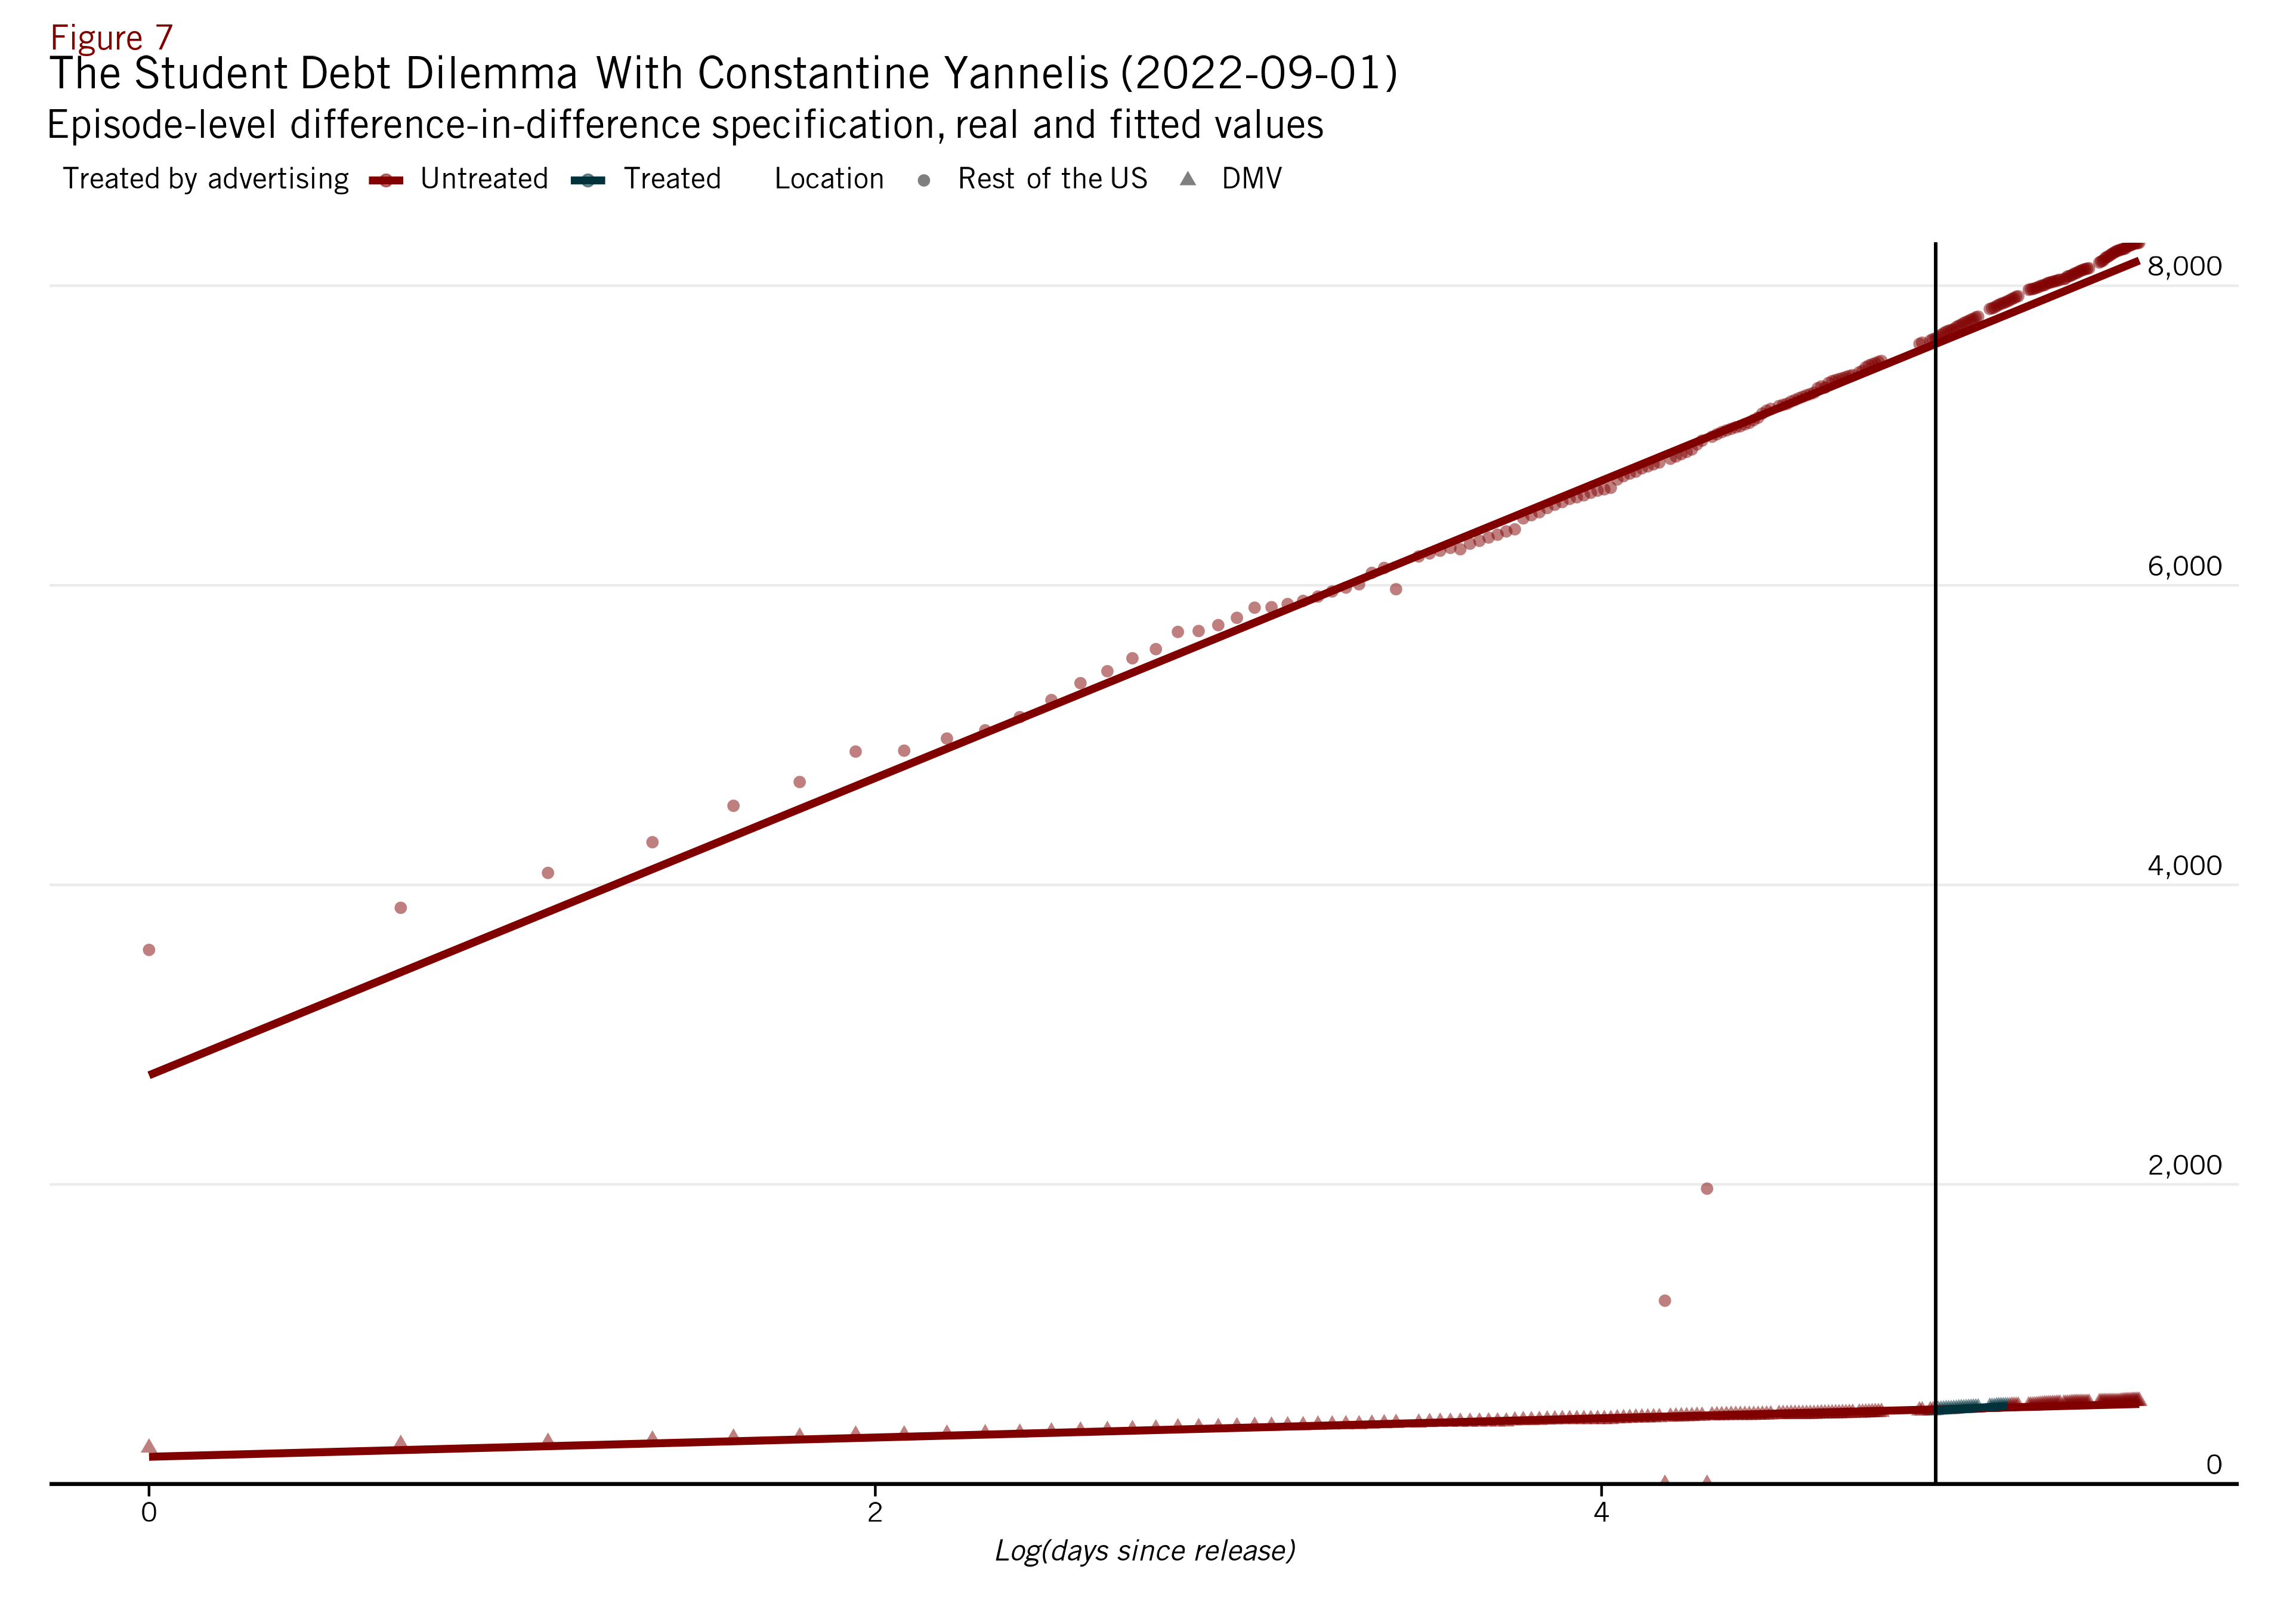
\includegraphics[width=0.9\textwidth]{figures/yannelis_did_whole_country_plot.png}
  \caption{}
  \label{fig:yannelis-did-RoUS}
\end{figure}

Figure \ref{fig:yannelis-did-RoUS} depicts the cumulative downloads performance of ``The Student Debt Dilemma with Constantine Yannelis,'' (published in September 2022), in the DMV area and in the rest of the United States. Note that in this setting only observations in the DMV area are every potentially treated because we restrict the definition of treatment to those places where the advertisement could plausibly have been seen. Importantly for the DID regression design, this episode clearly does not satisfy the ``parallel trends assumption,'' that is required to identify the causal effect of the advertising treatment. That is, the ``Rest of the United States'' is a poor control group for the DMV.\footnote{I repeat this exercise for the 50 most recent episodes and find that this is generally true --- the parallel trends assumption is rarely if every fully satisfied.} I conjecture that this is because long-run episode performance (long-run being the appropriate framing in this case because I am interested in cases where there is a clearly established performance trajectory for an episode) is a function of word-of-mouth dynamics in a very long-tail of ``small'' locations. That is, the DMV area is, to a greater or lesser extent, saturated to an extent that word-of-mouth dynamics do not take hold in an appreciable way.\footnote{Even disregarding the requirement for the parallel trends assumption to be satisfied, I find that the coefficient on the interaction term of interest ($\beta_5$) exhibits no meaningful degrees of statistical significance. Results of the visual parallel trends assumption test and regression results can be made available on request.}\\

In an effort to remedy this, I restrict the definition of the ``control'' group to only locations in New York state. Comparing a metropolitan area to a large state might still exhibit the same problem as outlined above but it is likely to be considerably attenuated because there are fewer such ``small'' places that can incidentally discover the podcast/epsiode for the first time (well after release). Additionally, in a subsequent set of regressions, I restrict the time sample under consideration to the 45 days prior-to and following the beginning of the advertising campaign. I do this to, as much as possible, omit the earliest period of the episode's performance, when daily downloads are relatively volatile (are by themselves the least predictive of long-run performance). Consider, for example, Figure \ref{fig:yannelis-did-nys}. Though not yet perfectly, the redefinition of the control group appears to better satisfy the parallel trends assumption and, encouragingly, a visual inspection suggests that advertising may have had a positive effect on podcast performance.\\

\begin{figure}[!htb]
  \centering
  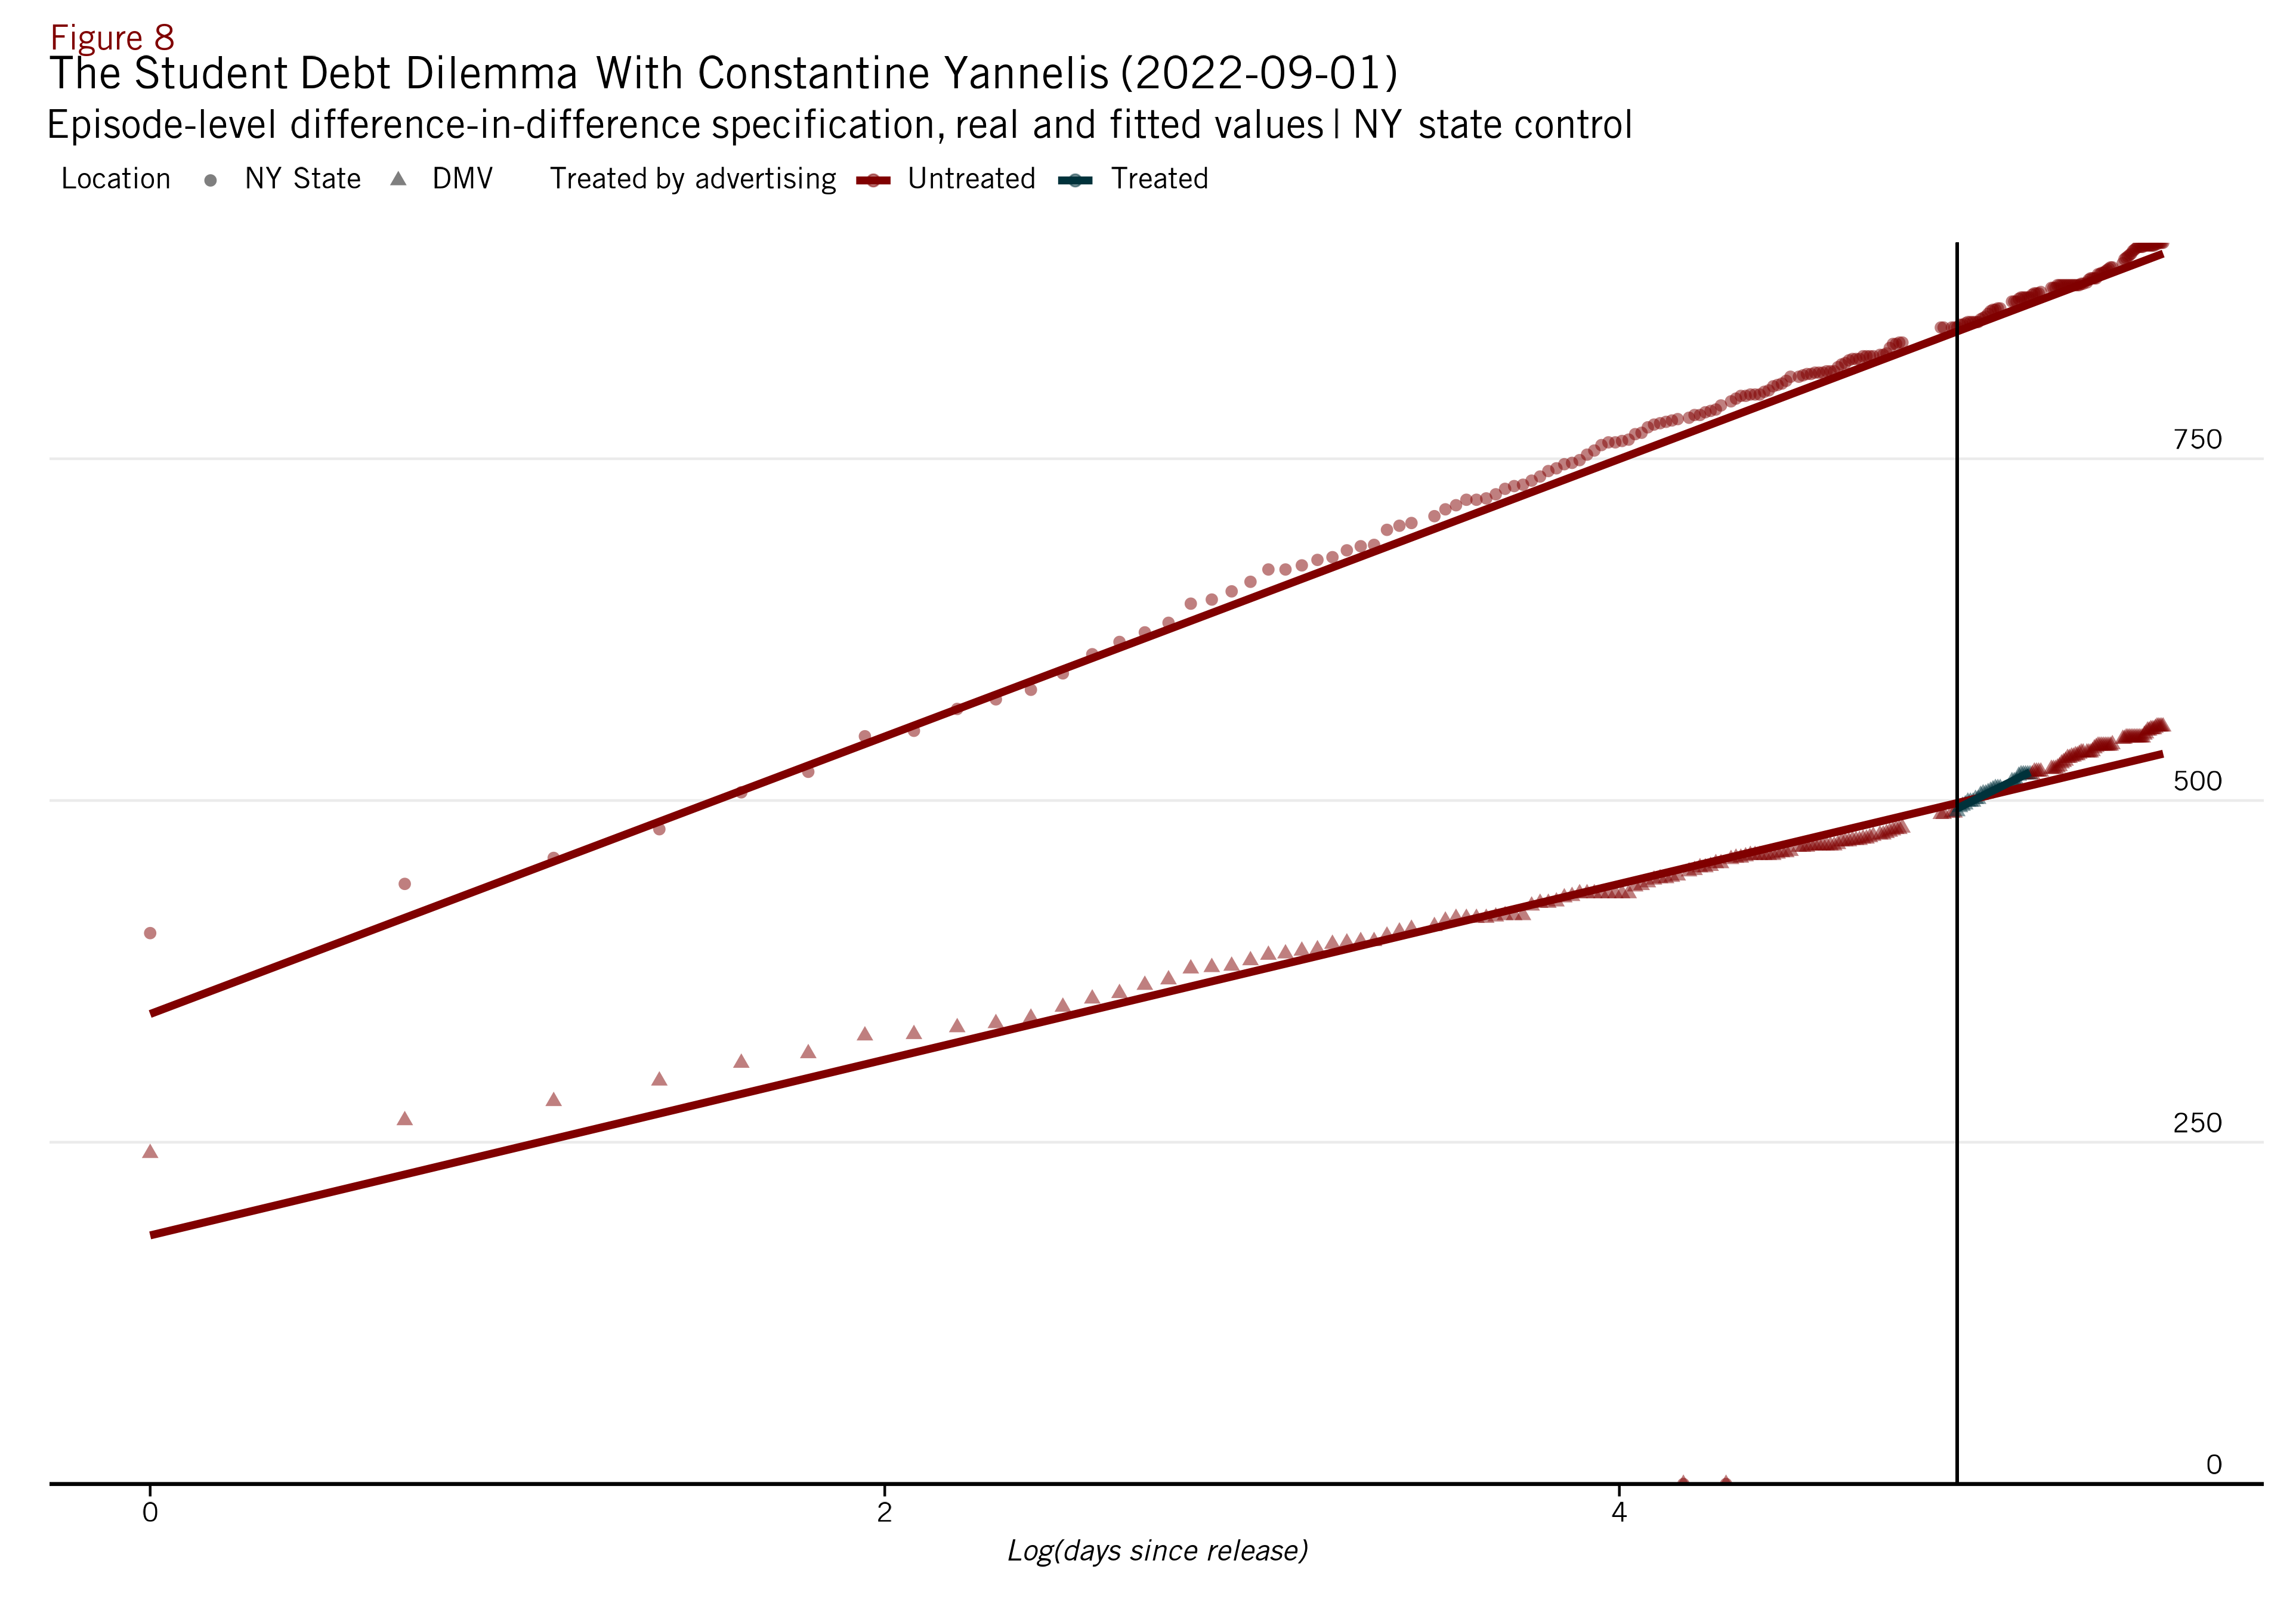
\includegraphics[width=0.9\textwidth]{figures/yannelis_did_nys_plot.png}
  \caption{}
  \label{fig:yannelis-did-nys}
\end{figure}

Closer inspection of the regression estimates, however, suggest that this is not the case. When restricting the control group to be only New York state, the coefficient on the interaction term remains statistically insignificant at the usual thresholds of interest. If I additionally restrict the time period under consideration to 45 days preceding and following the WMATA campaign beginning, however, these results change very slightly. The coefficient on the interaction term becomes statistically significant at the 5\% level but its magnitude remains very small: 0.0306. Compared to coefficient on the DMV-specific pre-trends, 97.49 cumulative downloads per unit log-day units, this constitutes an approximately 0.03\% increase in download performance --- effectively economically insignificant.\\

Turning our attention to other episodes, however, even this partially encouraging result fails to materialize. Table \ref{tab:dmv-nys-did-results} presents estimated values for \eqref{dmv-did} for the eight episodes released prior to the beginning of the advertising period, those that are most likely to experience the largest treatment effect to advertising, given that they are the episodes in the back catalog that are most likely to be seen by new listeners.

\begin{landscape}
  \begin{table}

\caption{Episode-level Difference-in-Difference Estimates, Selected Episodes}
\centering
\begin{tabular}[t]{l>{\centering\arraybackslash}p{0.76in}>{\centering\arraybackslash}p{0.76in}>{\centering\arraybackslash}p{0.76in}>{\centering\arraybackslash}p{0.76in}>{\centering\arraybackslash}p{0.76in}>{\centering\arraybackslash}p{0.76in}>{\centering\arraybackslash}p{0.76in}>{\centering\arraybackslash}p{0.76in}}
\toprule
  & Meritoracy Rerun & King 2 & Doctorow & Ramaswamy Rerun & Musk & Cochrane & Piketty & Antitrust-Isn't\\
\midrule
\addlinespace[0.5em]
\multicolumn{9}{l}{\textit{Full time sample:}}\\
\midrule \hspace{1em}$\log$ DaysSinceRelease & 127.841*** & 113.902*** & 116.534*** & 137.709*** & 109.183*** & 120.253*** & 146.334*** & 143.554***\\
\hspace{1em} & (2.901) & (4.100) & (1.968) & (9.304) & (0.646) & (0.909) & (8.721) & (4.148)\\
\hspace{1em}DMV & -141.648*** & -100.580*** & -162.465*** & -74.516 & -158.496*** & -184.775*** & -116.824* & -114.595***\\
\hspace{1em} & (18.225) & (25.465) & (11.333) & (49.638) & (5.086) & (6.774) & (47.323) & (25.117)\\
\hspace{1em}Advertisement & 8.714* & -7.909* & -10.496*** & -8.576* & 1.442** & -5.693*** & -1.295 & 12.779**\\
\hspace{1em} & (3.552) & (3.949) & (1.885) & (3.634) & (0.547) & (0.625) & (3.589) & (4.313)\\
\hspace{1em}DMV Pre-trends & -37.870*** & -46.907*** & -45.819*** & -60.732*** & -43.136*** & -38.152*** & -51.497*** & -58.847***\\
\hspace{1em} & (4.217) & (5.752) & (2.559) & (10.918) & (1.133) & (1.372) & (10.059) & (4.907)\\
\hspace{1em}Interaction & -3.453* & -3.000* & -1.289* & -1.124 & -2.487*** & -0.838*** & -3.942*** & -6.274***\\
\hspace{1em} & (1.527) & (1.464) & (0.653) & (1.006) & (0.263) & (0.236) & (0.972) & (1.150)\\
\hspace{1em}Intercept & 256.897*** & 223.045*** & 351.673*** & 199.654*** & 380.914*** & 390.969*** & 250.633*** & 244.546***\\
\hspace{1em} & (12.469) & (18.129) & (8.668) & (42.310) & (2.887) & (4.208) & (40.957) & (21.400)\\
\hspace{1em}Num.Obs. & 188 & 200 & 226 & 252 & 280 & 308 & 336 & 362\\
\addlinespace[0.5em]
\multicolumn{9}{l}{\textit{45-day window:}}\\
\midrule \hspace{1em}$\log$ DaysSinceRelease & 126.789*** & 110.478*** & 112.150*** & 124.072*** & 113.580*** & 106.212*** & 140.728*** & 187.432***\\
\hspace{1em} & (2.975) & (5.165) & (2.774) & (1.139) & (0.889) & (1.272) & (1.377) & (1.257)\\
\hspace{1em}DMV & -145.360*** & -91.969*** & -158.446*** & -95.244*** & -173.599*** & -221.038*** & -214.337*** & -50.751**\\
\hspace{1em} & (19.766) & (23.987) & (10.800) & (8.837) & (8.478) & (8.541) & (17.567) & (19.036)\\
\hspace{1em}Advertisement & 3.058 & -3.852 & -3.124 & -4.455* & -0.182 & -2.868*** & 0.794 & 0.425\\
\hspace{1em} & (2.774) & (3.872) & (3.212) & (1.805) & (0.569) & (0.485) & (0.632) & (0.700)\\
\hspace{1em}DMV Pre-trends & -38.049*** & -52.268*** & -47.846*** & -57.235*** & -41.406*** & -30.669*** & -32.805*** & -75.691***\\
\hspace{1em} & (5.198) & (6.623) & (3.348) & (2.503) & (2.058) & (1.986) & (3.905) & (4.121)\\
\hspace{1em}Interaction & -2.102+ & 0.048 & -0.255 & 0.333 & -0.789* & -0.349 & -1.856*** & -2.713***\\
\hspace{1em} & (1.162) & (1.454) & (1.141) & (0.740) & (0.307) & (0.261) & (0.438) & (0.477)\\
\hspace{1em}Intercept & 265.879*** & 231.372*** & 361.625*** & 252.769*** & 363.250*** & 452.051*** & 274.865*** & 45.797***\\
\hspace{1em} & (11.511) & (18.871) & (9.168) & (4.214) & (3.851) & (5.756) & (6.376) & (5.835)\\
\hspace{1em}Num.Obs. & 80 & 92 & 118 & 128 & 128 & 128 & 128 & 128\\
\bottomrule
\multicolumn{9}{l}{\rule{0pt}{1em}+ p $<$ 0.1, * p $<$ 0.05, ** p $<$ 0.01, *** p $<$ 0.001}\\
\multicolumn{9}{l}{\rule{0pt}{1em}Standard errors are presented in parentheses are are heteroskedastic-robust errors}\\
\end{tabular}
\end{table}

\end{landscape}


\end{document}